\documentclass{article}
\usepackage[T1]{fontenc}
\usepackage{listings}
\usepackage[english, greek]{babel}
\usepackage{tikz}
\usepackage[intlimits]{amsmath}
\usepackage{commath}
\usepackage{amssymb}
\usepackage{graphicx}
\graphicspath{ {./plots/} }
\setlength{\parindent}{0pt}


\lstset{frame=tb,
  language=C,
  aboveskip=3mm,
  belowskip=3mm,
  showstringspaces=false,
  columns=flexible,
  basicstyle={\small\ttfamily},
  numbers=none,
  numberstyle=\tiny\color{gray},
  stringstyle=\color{mauve},
  breaklines=true,
  breakatwhitespace=true,
  tabsize=3
}

\begin{document}

\begin{titlepage}
   \vspace*{\stretch{1.0}}
   \begin{center}
      \selectlanguage{english}
   	  \Large\textbf{Algorithms Spring 2024}\\
   	  \selectlanguage{greek}
      \Large\textbf{\selectlanguage{english}Project Report\selectlanguage{greek}}\\
      \large\textit{Δημήτρης Παπαδημτρίου-Βασίλης Μαδέσης}\\
      \large\textit{AEM: 03750-03748}
   \end{center}
   \vspace*{\stretch{2.0}}
\end{titlepage}

\textbf{Τρόπος αποθήκευσης γράφων και δομές δεδομένων:}\bigbreak

Για την αποθήκευση του γράφου χρησιμοποιούμε έναν πίνακα απο λίστες γειτνίασης. Κάθε θέση του πίνακα δηλαδή αντοιστιχεί σε έναν κόμβο του γράφου, και περιέχει μία απλά συνδεδεμένη λίστα, κάθε στοιχείο της οποίας περιέχει 
έναν κόμβο με τον οποίο ο αρχικός συνδέεται. Γενικά οι λίστες γειτνίασης χρησιμοποιούνται για αλγορίθμους γράφων όπως \selectlanguage{english} Breadth First Search\selectlanguage{greek} που χρησημοποιήσαμε και στην άσκηση,
και είναι πολύ αποδοτικές σε αραιούς γράφους, όπως αυτούς που δώθηκαν στα παραδείγματα.
Άλλες δομές δεδομένων που χρησιμοποιήθηκαν στο πρόγραμμα είναι οι πίνακες, για να αποθηκεύσουμε για παράδειγμα την απόσταση καθώς και τις χρήσεις σε συντομότερα μονοπάτια για κάθε ακμή, και οι ούρες, που αποτελούν κομμάτι
του \selectlanguage{english} Breadth First Search\selectlanguage{greek} αλγόριθμου.\bigbreak

\textbf{Εύρεση \selectlanguage{english}CPL\selectlanguage{greek} ενός γράφου:}\bigbreak

Για να βρούμε το \selectlanguage{english}CPL\selectlanguage{greek} ενός γράφου χρησημοποιήσαμε\selectlanguage{english} Breadth First Search\selectlanguage{greek} ώστε να υπολογίσουμε όλα τα μήκοι των σύντομων μονοπάτιων μεταξύ όλων των κόμβων.Συγκεκριμένα υλοποιούμε μια συνάρτηση η οποία λαμβάνει ως \selectlanguage{english}input\selectlanguage{greek} το \selectlanguage{english}source node\selectlanguage{greek} και έχει ένα πίνακα που κρατάει τις αποστάσεις όλων των κόμβων από τον κόμβο \selectlanguage{english}source\selectlanguage{greek} μαζί με ένα πίνακα με τους γονείς κάθε κόμβου.Ο πίνακας γονιών θα χρησιποιηθεί αργότερα για το Β ερώτημα όπου θα εξηγήσουμε την χρήση του.Τελός η συνάρτηση αυτή επιστρέφει τους πίνακες αύτους ενώ αν της δωθεί συγκεκριμένος \selectlanguage{english}destination\selectlanguage{greek} κομβός τότε θα τρέχει μέχρι να βρεί το κόμβο αυτό επιστρέφοντας επιτυχία με 1 και αποτυχία με 0.\bigbreak

Για την υλοποίηση της \selectlanguage{english} Breadth First Search\selectlanguage{greek} χρήσιμοποιήουμε μια \selectlanguage{english}queue (FIFO \selectlanguage{greek}ούρα) ώστε να τοποθετούμε μέσα της τους κόμβους που πρέπει να επισκεφτούμε μετά από μια επίσκεψη κόμβου σε κάθε επανάληψη.\pagebreak

Η συνάρτηση λειτουργεί ως εξής:

\selectlanguage{english}
\begin{lstlisting}
pathSearch()
distance[size of graph] -> 0

Insert in queue node S
while(Queue is not empty)
	parent node <- remove from queue the first element
	
	for all child nodes of parent node
		if(distance[child node] is 0 && child node != S)
			Put child node into queue
			distance[child node] = distance[parent node] + 1
			parent[child node] = parent node
		else if(distance[child node] == distance[parent node] + 1)
			parent[child node] -> add parent to the list of parents for child node
		if (distance[child node] == distance[parent node] + 1 && child node == destination node)
			return 1
	end	
return 0
end
\end{lstlisting}\bigbreak
\selectlanguage{greek}

Για να βρούμε το \selectlanguage{english}CPL\selectlanguage{greek} εκτελούμε κατα επανάληψη την προηγούμενη συνάρτηση για όλους τους κόμβους και μηδενίζουμε τις επαναλαμβανόμενες αποστάσεις που προκύπτουν στον πίνακα αποστάσεων που μας επιστρέφει η συνάρτηση και έπειτα προσθέτουμε στο συνολικό άθροισμα, το άθροισμα των αποστάσεων του πίνακα αυτού.\bigbreak
Τέλος για να βρούμε το συνολικό \selectlanguage{english}CPL\selectlanguage{greek} παίρνουμε το άθροισμα στο τέλος της επανάληψης και το διαιρούμε με το πλήθος των ζευγαριών κόμβων.

\selectlanguage{english}
\begin{lstlisting}
Sum of all cpls = 0;

for all nodes inside the graph
	distances array = execute pathSearch
	distances array -> distance array with zeroed the recurring distances
	Sum of all cpls = distances array + Sum of all cpls
end

cpl = Sum of all cpls / binomial coefficient(number of nodes,2)
\end{lstlisting}\pagebreak
\selectlanguage{greek}

\textbf{Υπολογισμός \selectlanguage{english}SPs\selectlanguage{greek} που μεσολαβεί από μια ακμή $e$}\bigbreak

Για να υπολογίσουμε τον συνολικό αριθμό των συντομοτέρων μονοπατιών \selectlanguage{english}(SPs)\selectlanguage{greek} μεταξύ κάθε δυνατού ζεύγους κόμβων $j$ και $k$ στα οποία μεσολαβεί κάθε ακμή $e$ του γραφήματος.Θα χρησιμοποιήσουμε τον πίνακα γονέων που μας επιστρέφει η συνάρτηση
\selectlanguage{english}pathSearch()\selectlanguage{greek}.\bigbreak

Ο πίνακας γονέων είναι ένας πίνακας που σε κάθε θέση $i$ έχει τον γονέα του κόμβου $i+1$.Γονέας ενός κόμβου είναι ο γειτονικός κόμβος από τον οποίο διαβάστηκε και μπήκε στον πίνακα αποστάσεων ο κόμβος παιδί(στην περιπτωσή μας ο κόμβος $i+1$).Σε περίπτωση ύπαρξης δύο ή περισσότερων σύντομων μονοπατιών μεταξύ δύο κόμβων ο κόμβος \selectlanguage{english}destination\selectlanguage{greek} θα έχει δύο γονείς καθώς και οι δύο είναι μέρος σύντομου μονοπατιού.\bigbreak

Οι συμλήρωση του πίνακα γονέων φαίνεται στο παρακάτω \selectlanguage{english}code snippet\selectlanguage{greek} της συνάρτησης\selectlanguage{english} pathSearch\selectlanguage{greek}:

\selectlanguage{english}
\begin{lstlisting}
if(distance[child node] is 0 && child node != S)
			Put child node into queue
			distance[child node] = distance[parent node] + 1
			parent[child node] = parent node
else if(distance[child node] == distance[parent node] + 1)
			parent[child node] -> add parent to the list of parents for child node
\end{lstlisting}\bigbreak
\selectlanguage{greek}
\bigbreak
Αν ο κόμβος έχει παραπάνω από έναν γονέα τότε δημιουργείται μια λίστα με του γονείς του κόμβου αυτού στην αντίστοιχη θέση του πίνακα.\bigbreak

Προσθέτοντας στον προήγουμενο κώδικα, για κάθε επανάληψη της 'λούπας' παίρνουμε τον πίνακα γονέων και για κάθε ζευγάρι κόμβων\selectlanguage{english} source-destination\selectlanguage{greek} διατρέχουμε το πίνακα ξεκίνοντας από το \selectlanguage{english}destination\selectlanguage{greek} και ακολουθώντας τον γονέα του και από εκεί ακολουθώντας τον γονέα του γονέα του ,φτάνουμε στο \selectlanguage{english}source\selectlanguage{greek} καταγράφοντας τα \selectlanguage{english}edges\selectlanguage{greek} που συμμετείχαν στο δρόμο μέχρι το \selectlanguage{english}source\selectlanguage{greek}.\pagebreak

Το \selectlanguage{english}path\selectlanguage{greek} για κάθε ζεύγος καθώς και τα \selectlanguage{english}edges\selectlanguage{greek} που συμμετέχουν σε αυτό βρίσκεται από τον ψευδοκώδικα:

\selectlanguage{english}
\begin{lstlisting}
countEdgesPath()
	current node = destination node
	while(parent of current node != Source)
	  array of edges [parent node][current node] ++
	  array of edges [parent node][current node] ->add info about the edge
	end
	
	if (there are more than one parents for destination node)
		repeat the process for the other parent of destination node
end
\end{lstlisting}
\selectlanguage{greek}

Ο συνολικός ψευδοκώδικας προκύπτει:
\bigbreak
\selectlanguage{english}

\begin{lstlisting}
Sum of all cpls = 0;

for all nodes inside the graph
	distances array = execute pathSearch
	distances array -> distance array with zeroed the recurring distances
	Sum of all cpls = distances array + Sum of all cpls
	
	for all combinations of sources and destination nodes inside a graph
		countEdgesPath() fill the edge array
	end 
end

cpl = Sum of all cpls / binomial coefficient(number of nodes,2)
\end{lstlisting}\bigbreak
\selectlanguage{greek}

Τέλος έξω απο την επανάληψη κάνουμε \selectlanguage{english}merge sort\selectlanguage{greek} το πίνακα \selectlanguage{english}edge array\selectlanguage{greek} και επιστρέφουμαι το πρώτο \selectlanguage{english}edge\selectlanguage{greek} του πίνακα το οποίο και θα αφαιρέσουμε.Το δύο προηγούμενα ερωτήματα τα εκτελεί η συνάρτηση \selectlanguage{english}cpl sp\selectlanguage{greek}.\pagebreak

\selectlanguage{english}
\begin{lstlisting}
cpl_sp()
Sum of all cpls = 0;

for all nodes inside the graph
	distances array = execute pathSearch
	distances array -> distance array with zeroed the recurring distances
	Sum of all cpls = distances array + Sum of all cpls
	
	for all combinations th source and destination nodes inside the graph
		countEdgesPath() fill the edge array
	end 
end

cpl = Sum of all cpls / binomial coefficient(number of nodes,2)
mergesort(edge array)

return top elemnent in edge array
end
\end{lstlisting}\bigbreak
\selectlanguage{greek}

Συνεπώς το \selectlanguage{english}complexity\selectlanguage{greek} της συνάρτησης προκύπτει ως εξής:\bigbreak

To \selectlanguage{english}complexity\selectlanguage{greek} της αναζήτησης είναι $Ο(V+E)$ όπου $V$ κόμβοι και $Ε$ ακμές.\bigbreak

Για την συνάρτηση μηδενισμού έχουμε \selectlanguage{english}complexity\selectlanguage{greek}
$O(V)$ όπως το ίδιο και για την συνάστηση αθροίσματος.\bigbreak

Η συνάστηση επαναληπτική εκτέλεση της συνάστησης\selectlanguage{english}countEdgesPath()\selectlanguage{greek} έχει \selectlanguage{english}comlexity\selectlanguage{greek}
$O(V*Biggest Path Length)$ καθώς εκτελείται περίπου $Ο(V)$ φορές για ένα δεδομένο πίνακα γονέων και η διάτρεξη του πίνακα γονέων έχει στην μεγαλύτερη περίπτωση μεταξύ όλων των $Ο(Biggest Path Length)$ πράξεις.\bigbreak

Άρα το συνολικό \selectlanguage{english}complexity\selectlanguage{greek} εφόσον γίνονται $V$ επαναλήψης είναι 

$Ο(V) * [O(V+E)+O(V)+O(V)+Ο(V*Biggest Path Length)] \ = \ O(V^2 + VE)$\bigbreak

Eφόσον έχουμε εκτελέσει την συνάρτηση \selectlanguage{english}cpl sp\selectlanguage{greek} τότε κάνουμε αφαίρεση της ακμής μεταξύ των δύο κόμβων αφαιρόντας τις μεταξύ ακμές από τις αντίστοιχες λίστες γειτνίασης τους.\pagebreak

\textbf{Αφαίρεση της ακμής, έλεγχος συνεκτικότητας του γράφου:}\bigbreak

Για την αφαίρεση της ακμής που ενώνει δύο κόμβους $i$, $j$, θα χρειασεί απλώς να αφαιρέσουμε τον κόμβο $j$ απο τη λίστα γειτνίασης του κόμβου $i$ και αντίστροφα.
Θα χρειαστεί όμως, όταν αφαιρεθεί η ακμή, να ελέγξουμε άν ο γράφος είναι συνεκτικός, η αν έχει χωριστεί σε δύο διαφορετικές συνιστώσες. 
Όμως, άν ο γράφος έχει πράγματι χωριστεί, σημαίνει πως η ακμή που αφαιρέσαμε ήταν ο μόνος συνεκτικός "κρίκος" ανάμεσα στους δύο γράφους.
Δηλαδή μπορούμε να διαπιστώσουμε άν οι γράφοι χωρίστηκαν, αρχίζοντας απο τον ένα κόμβο και ψάχνοντας τουλάχιστον ένα μόνοπάτι που θα οδηγήσει στον άλλον.
Προφανώς αν το μονοπάτι αυτό δέν υπάρχει, τότε σημαίνει πως οι γράφοι πράγματι χωρίστηκαν.
Η συνάρτηση \selectlanguage{english}Path search()\selectlanguage{greek} μπορεί να χρησιμοποιηθεί για την εύρεση αυτού του μονοπατιού, που επιστρέφει ανάλογη τιμή αν
βρεί τον \selectlanguage{english}destination node\selectlanguage{greek}. Θα μας δώσει επίσης τον πίνακα με τις αποστάσεις απο τον αρχικό κομβο 
\selectlanguage{english}(source node)\selectlanguage{greek}, που θα φανεί ιδιαίτερα χρήσιμο στο επόμενο βήμα του αλγορίθμου.\bigbreak
Η περιπλοκότητα αφαίρεσης ενός κόμβου θα κριθεί απο τον μέγιστο μέγεθος μίας λίστας γειτνίασης, δηλαδή είναι ίση με $Ο(V)$. Όμως επειδή οι γράφοι στα παραδείγματα 
είναι αραιοί, η περιπλοκότητα εδώ θα είναι στη πραγματικότητα αμελητέα.
Επίσης η περιπλοκότητα της αναζήτησης αντιστοιχεί στη περιπλοκότητα μιας επανάληψης του \selectlanguage{english} Breadth First Search\selectlanguage{greek}
αλγορίθμου, δηλαδή είναι ίση με $Ο(V + Ε)$ \bigbreak

\textbf{Αναδρομική συνάρτηση:}\bigbreak

Εδώ αξίζει να σημειωθεί η δομή της συνάρτησης που χρήσιμοποιείται, η οποία αποτελείται απο μία επανάληψη μέσα στην οποία καλούνται οι συναρτήσεις για την εύρεση του
\selectlanguage{english}cpl\selectlanguage{greek}, την αφαίρεση ενός κόμβου, τον έλεγχο συνεκτικότητας του γράφου καθώς και για την δημιουργία των δύο υπογράφων και
την αναδρομική κλίση του εαυτού της για καθέναν απο τους υπογράφους, αν χρειαστεί. Η αναδρομή τερματίζει όταν μια συνιστώσα αποτελείται απο έναν μονάχα κόμβο.
Αυτό φαίνεται και στον παρακάτω ψευδοκώδικα:\bigbreak

\selectlanguage{english}
\begin{lstlisting}
void analyseGraph():
	if numVertices = 1	
		return
	
	while 1:
		MostUsedEdge = cpl_sp()
		removeEdge(MostUsedEdge)
		
		is graph connected = pathSearch()

		if graph is not connected:
		
			subgraphs = splitGraph()
			analyseGraph(bigger subgraph)								
			analyseGraph(smaller subgraph)				
			return
\end{lstlisting}\bigbreak\selectlanguage{greek}

Για να δημιουργήσουμε τους υπογράφους, ιδιαίτερα χρήσιμος θα φανεί ο πίνακας αποστάσεων της \selectlanguage{english}pathSearch\selectlanguage{greek},
καθώς παρέχει έναν εύκολο τρόπο να ξεχωρίσουμε τους κόμβους που θα είναι μέρος κάθε υπογράφου. Συγκεκριμένα, κάθε κόμβος που αντιστoiχεί σε θέση του πίνακα
με απόσταση διάφορη του μηδενός, συμπεριλα-

μβανομένου του \selectlanguage{english}source node\selectlanguage{greek}, θα ανήκουν στον πρώτο γράφο, και τα 
υπόλοιπα θα ανοίκουν στον 2ο γράφο.\bigbreak

Όταν χωρίσουμε τους γράφους, χρησιμοποιούμε έναν αλγόριθμο για να αναπροσαρμόσει τους κόμβους στον κάθε καινούριο γράφο. Αρχικά τοποθετεί τους κόμβους του 
αρχικού γράφου που θα χρησιμοποιηθούν σε έναν πίνακα, όπου η θέση που θα τοποθετηθούν στον πίνακα αντιπροσωπεύει την ονομασία τους υπο τον καινούριο γράφο.
Έπειτα, για κάθε κόμβο που θα χρησιμοποιήσουμε, αντιγράφουμε κάθε στοιχείο της λίστας γειτνίασης, αλλάζοντας την "παλιά ονομασία" του κόμβου που αντιπροσωεύεται
με τη καινούρια. \bigbreak

\selectlanguage{english}\begin{lstlisting}
struct GraphPair splitGraph():

	new-order1 = all vertices for which dist != 0
	new-order1 = all vertices for which dist == 0

  	graph1 = reorderGraph(newOrder1)
  	graph2 = reorderGraph(newOrder2)
  
	return graps

\end{lstlisting}
\begin{lstlisting}
struct Graph* reorderGraph():
	newGraph = create Graph()

	for i in numVertices:

		while temp node of initial graph in new-order[i] list: 
			
			for j in numvertices:
				if new-order[j] = temp vertex:
					newDestIdx = j
					break

			addEdge(newDestIdx)
			temp = temp->next

	return newGraph

\end{lstlisting}\bigbreak\selectlanguage{greek}

Προφανώς η περιπλοκότητα αυτού του αλγορίθμου θα είναι ίση με $O(E)$, αφού θα προσπελάσουμε κάθε κόμβο του γράφου που θα σπάσουμε
Συνολικά η περιπλοκότητα μίας επανάληψης της αναδρομικής συνάρτησησς είναι ίση με το σύνολο των παραπάνω βημάτων δηλαδή με
$O(V^2 + VE) + O(V) + O(V + E) + O(E) \ = \ O(V^2 + VE)$ Επειδή όμως η επανάληψη θα εκτελεστεί για κάθε ακμή, δηλαδή $E$ φορές,
η συνολική περιπλοκότητα του αλγορίθμου θα είναι ίση με $O(ΕV^2 + VE^2)$, η καλύτερα $O(VE^2)$\bigbreak

\textbf{Τα \selectlanguage{english}plots\selectlanguage{greek}}\bigbreak

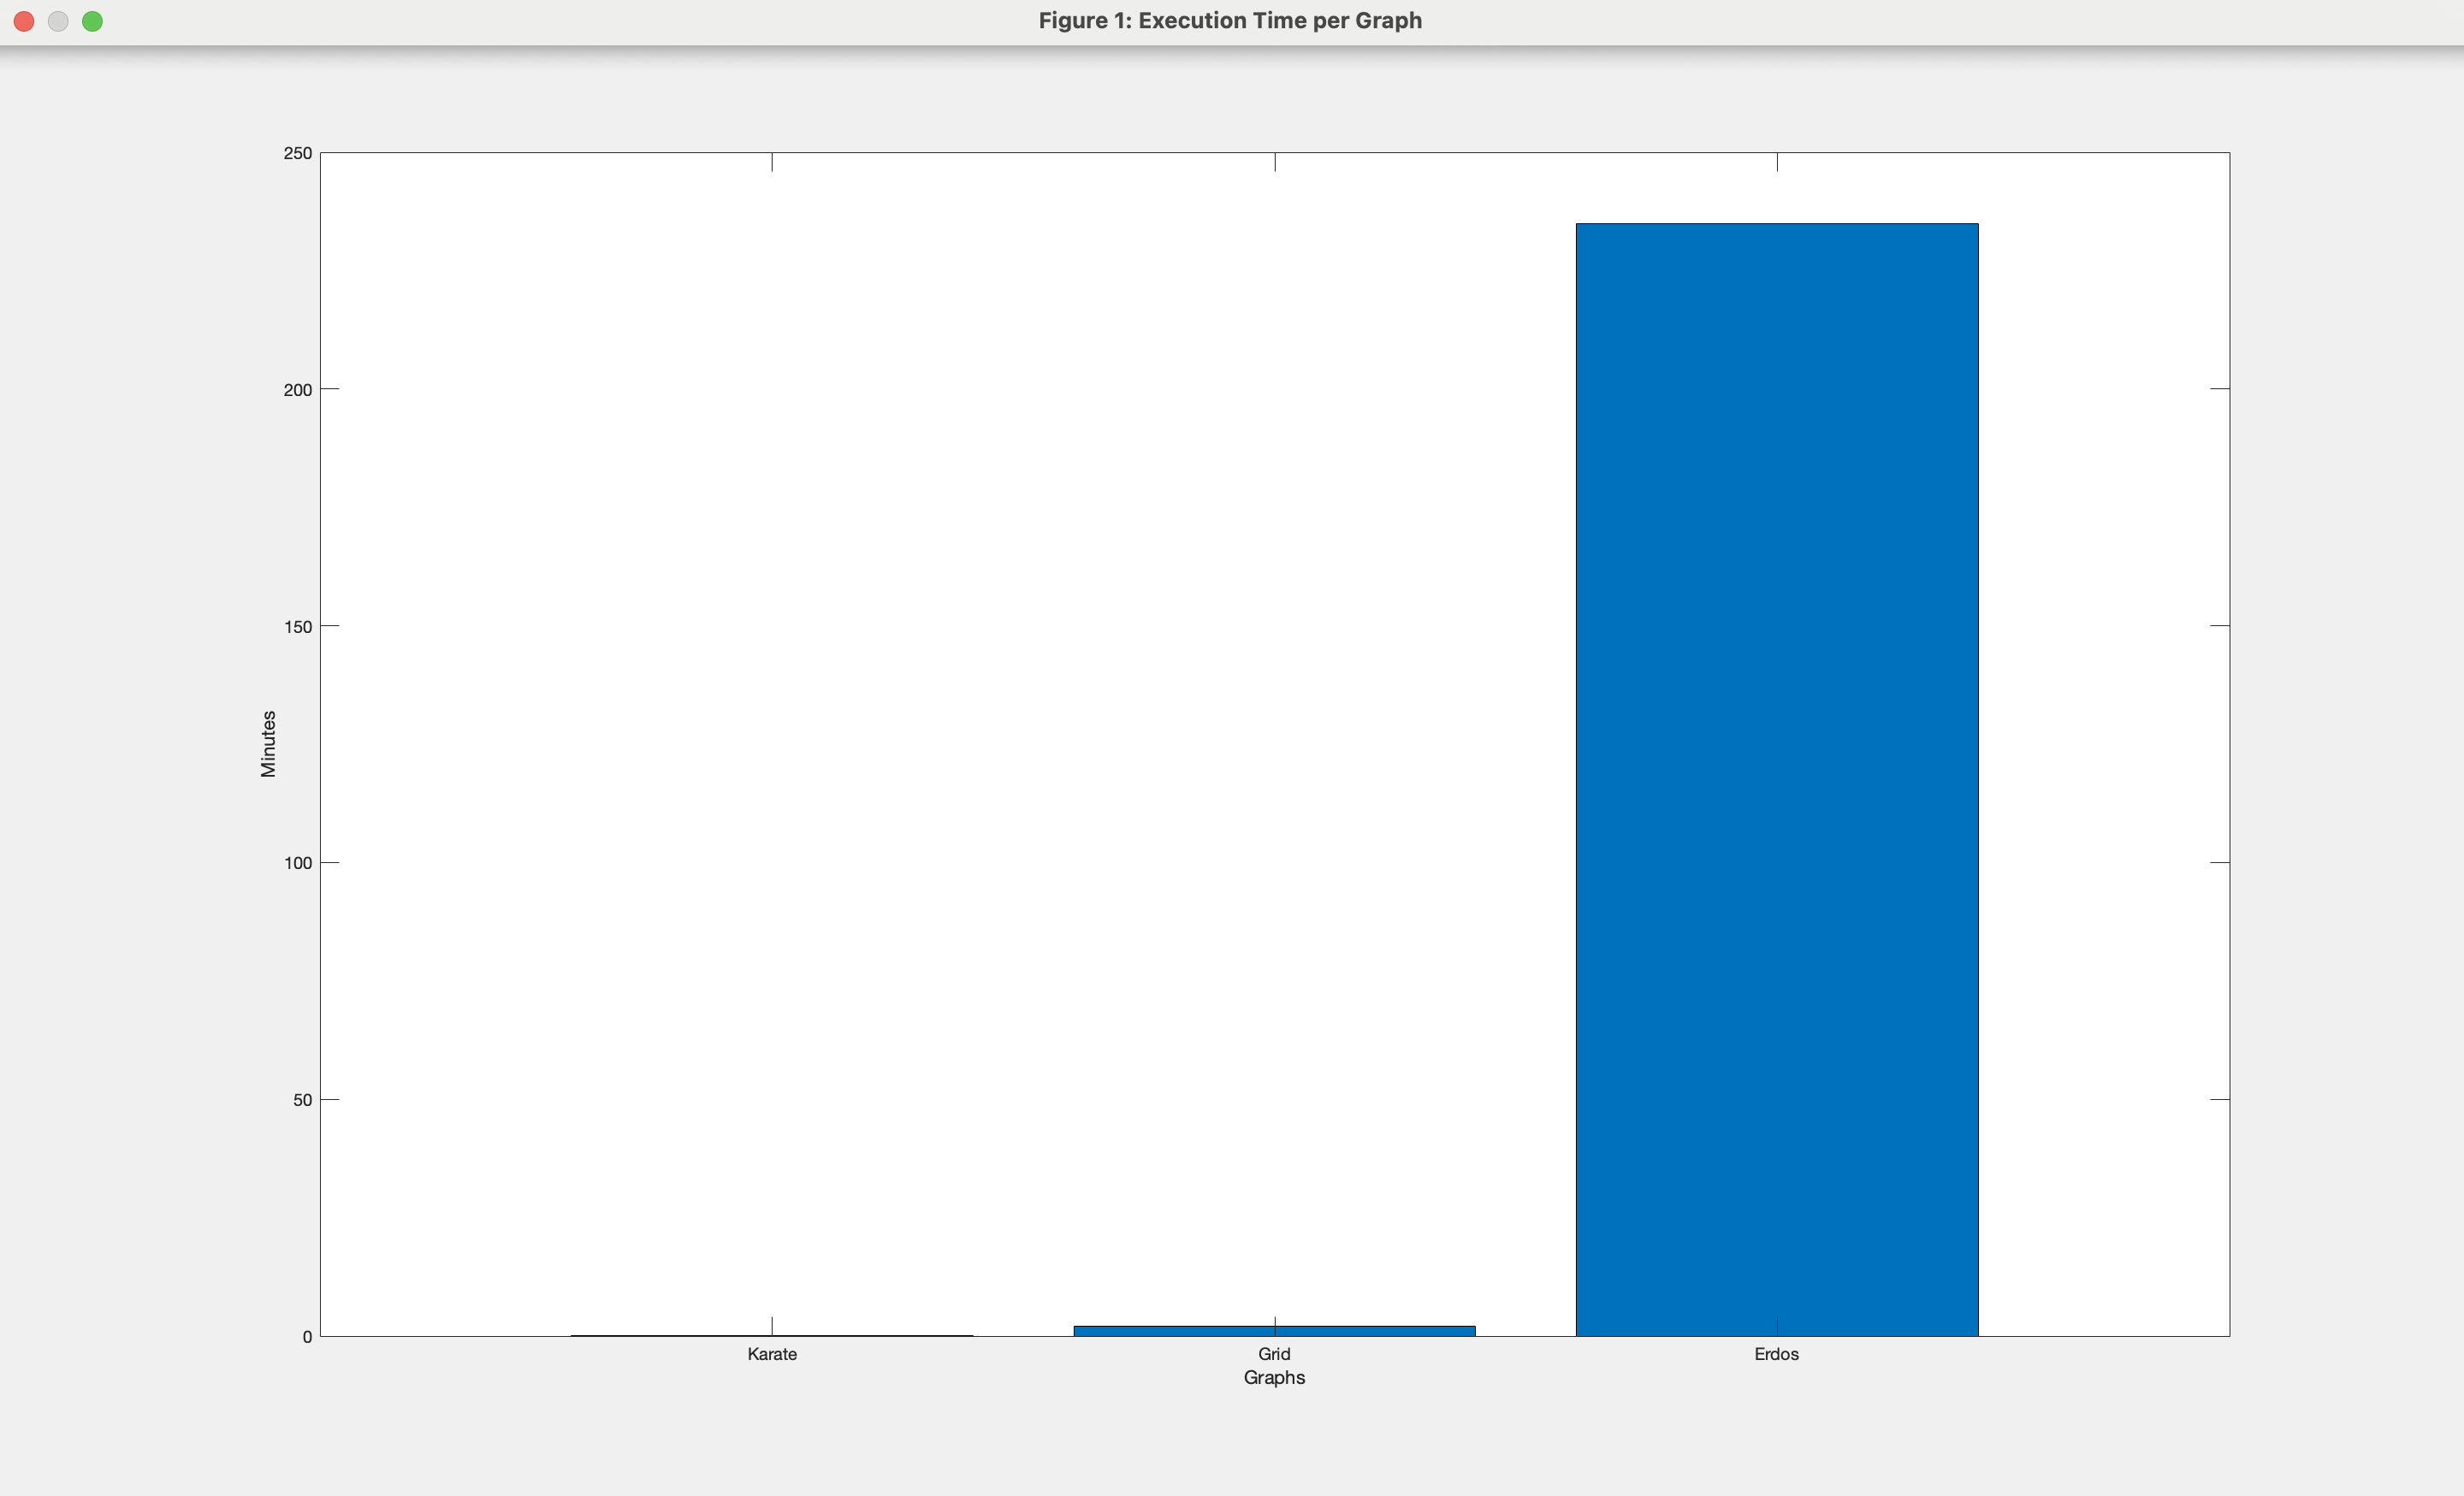
\includegraphics[width=\textwidth]{Figure1.png}\bigbreak
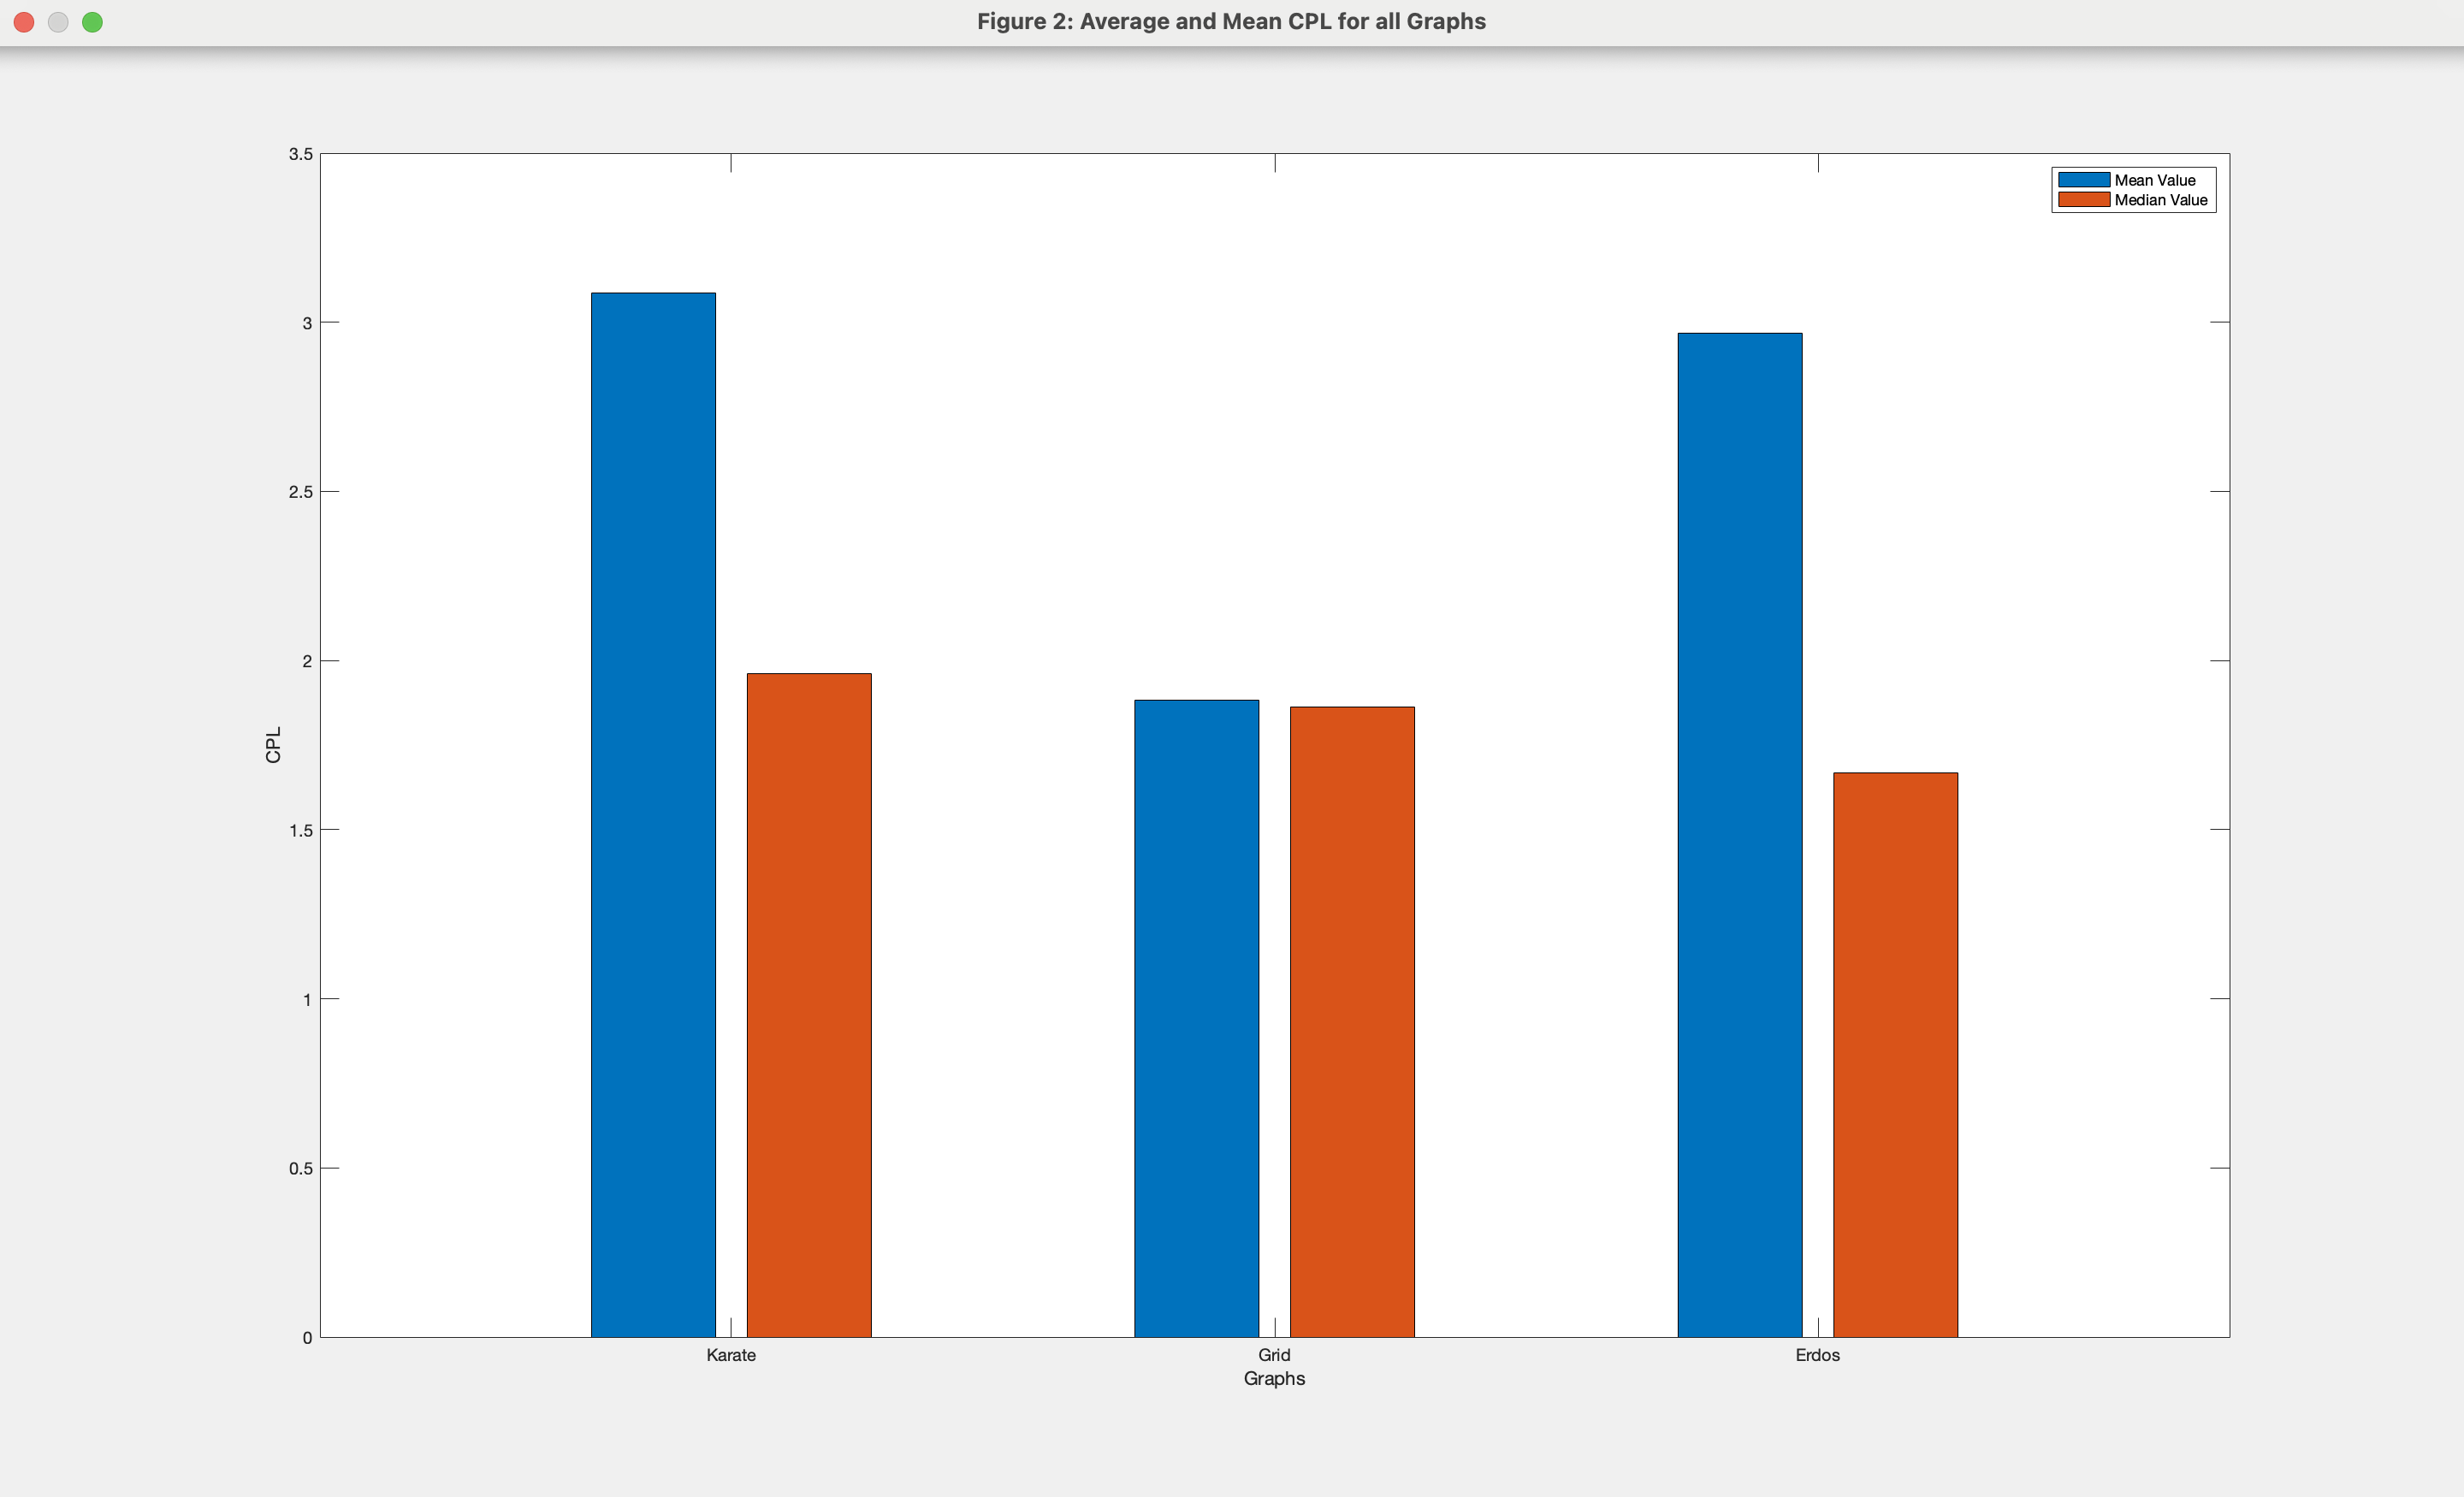
\includegraphics[width=\textwidth]{Figure2.png}\bigbreak
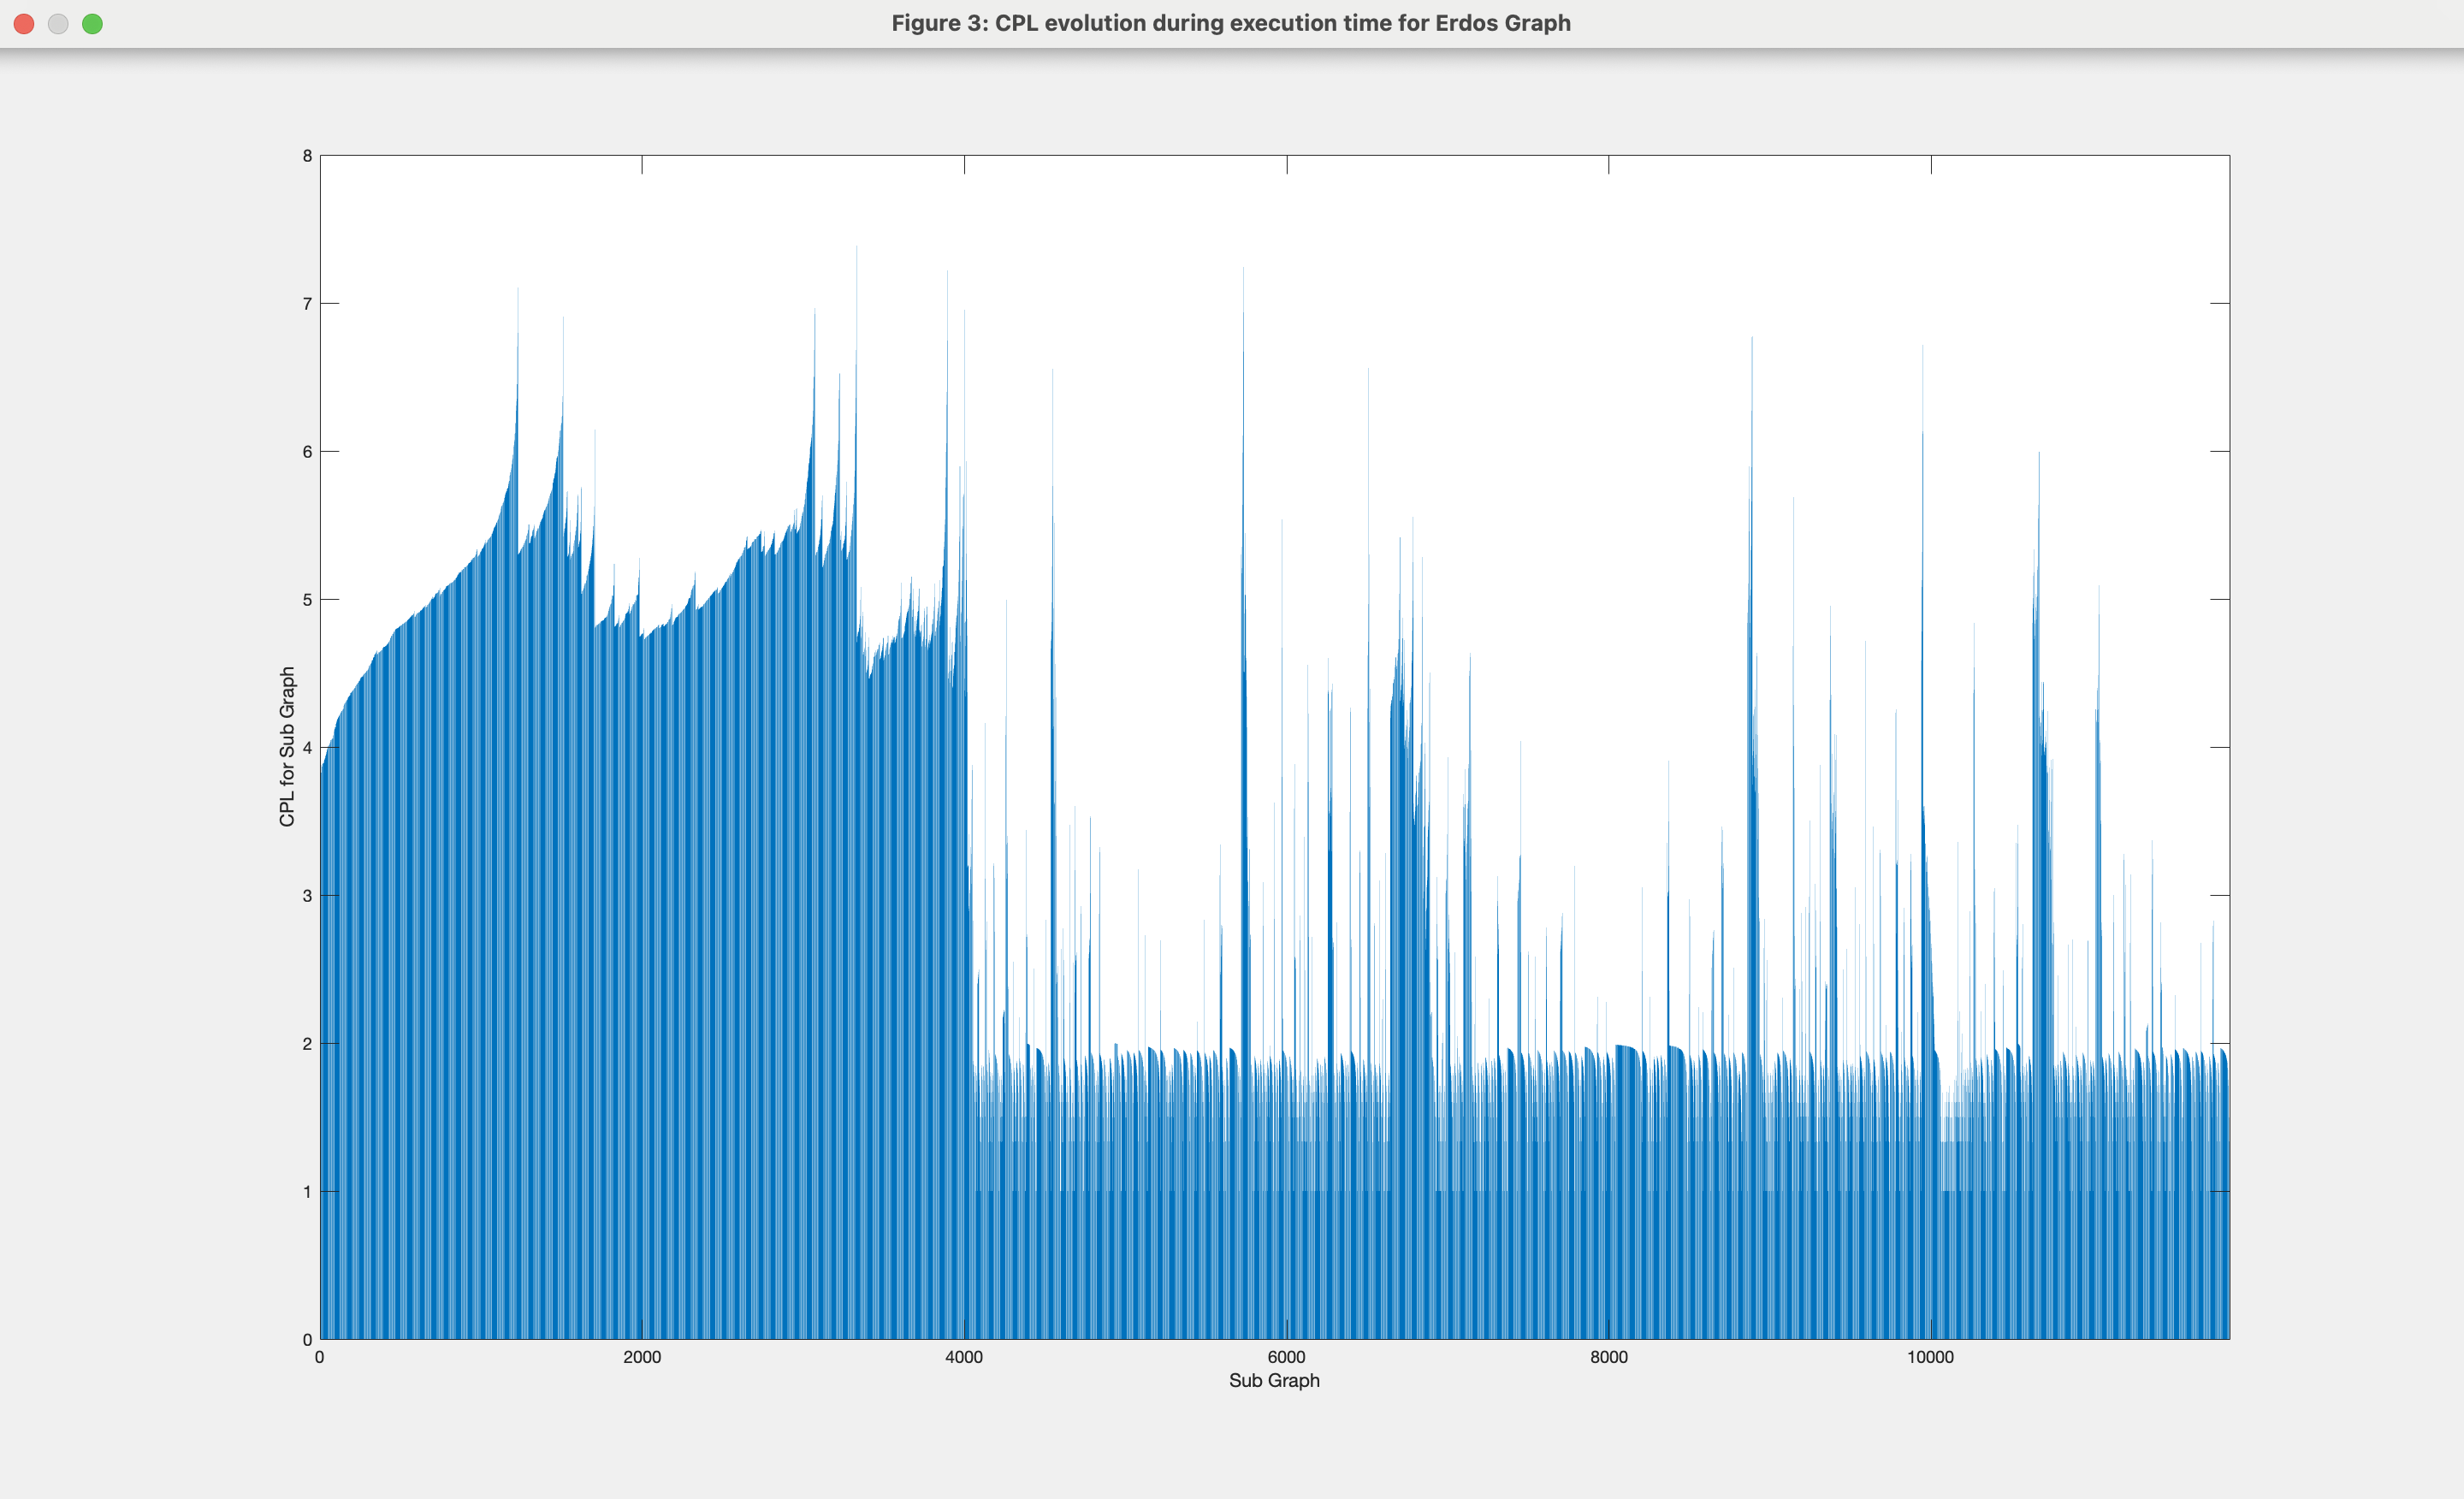
\includegraphics[width=\textwidth]{Figure3.png}\bigbreak
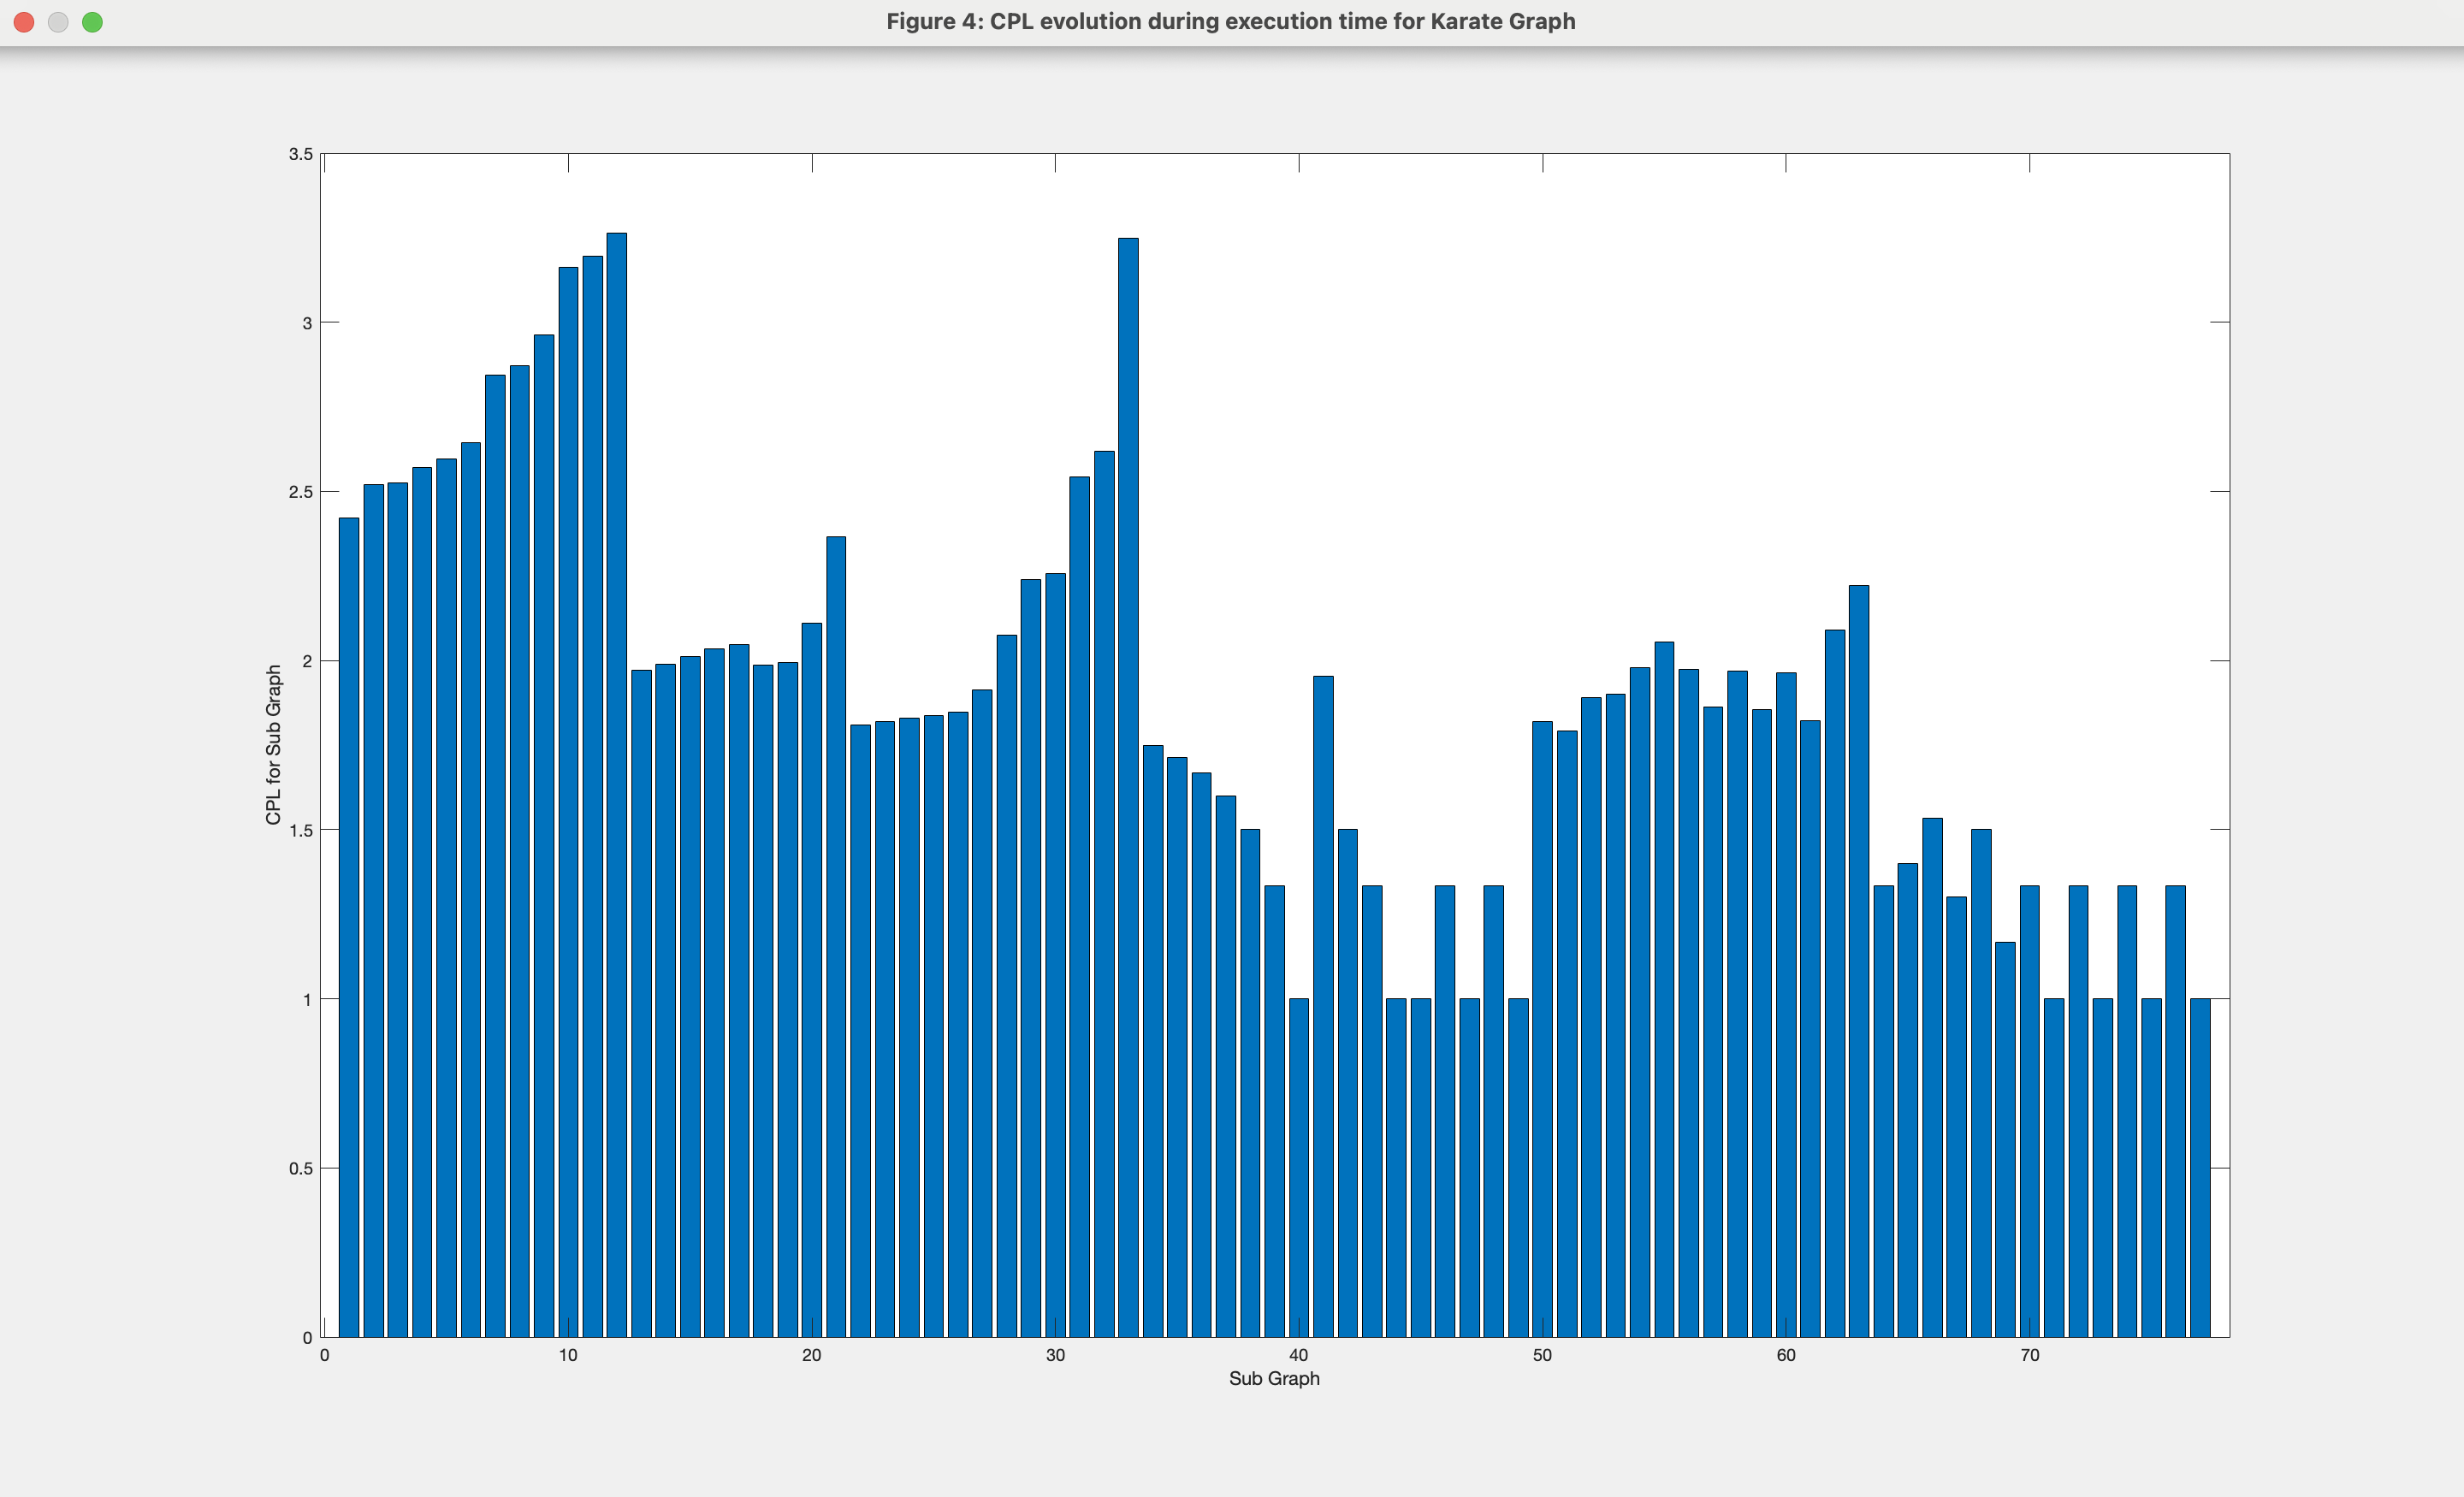
\includegraphics[width=\textwidth]{Figure4.png}\bigbreak
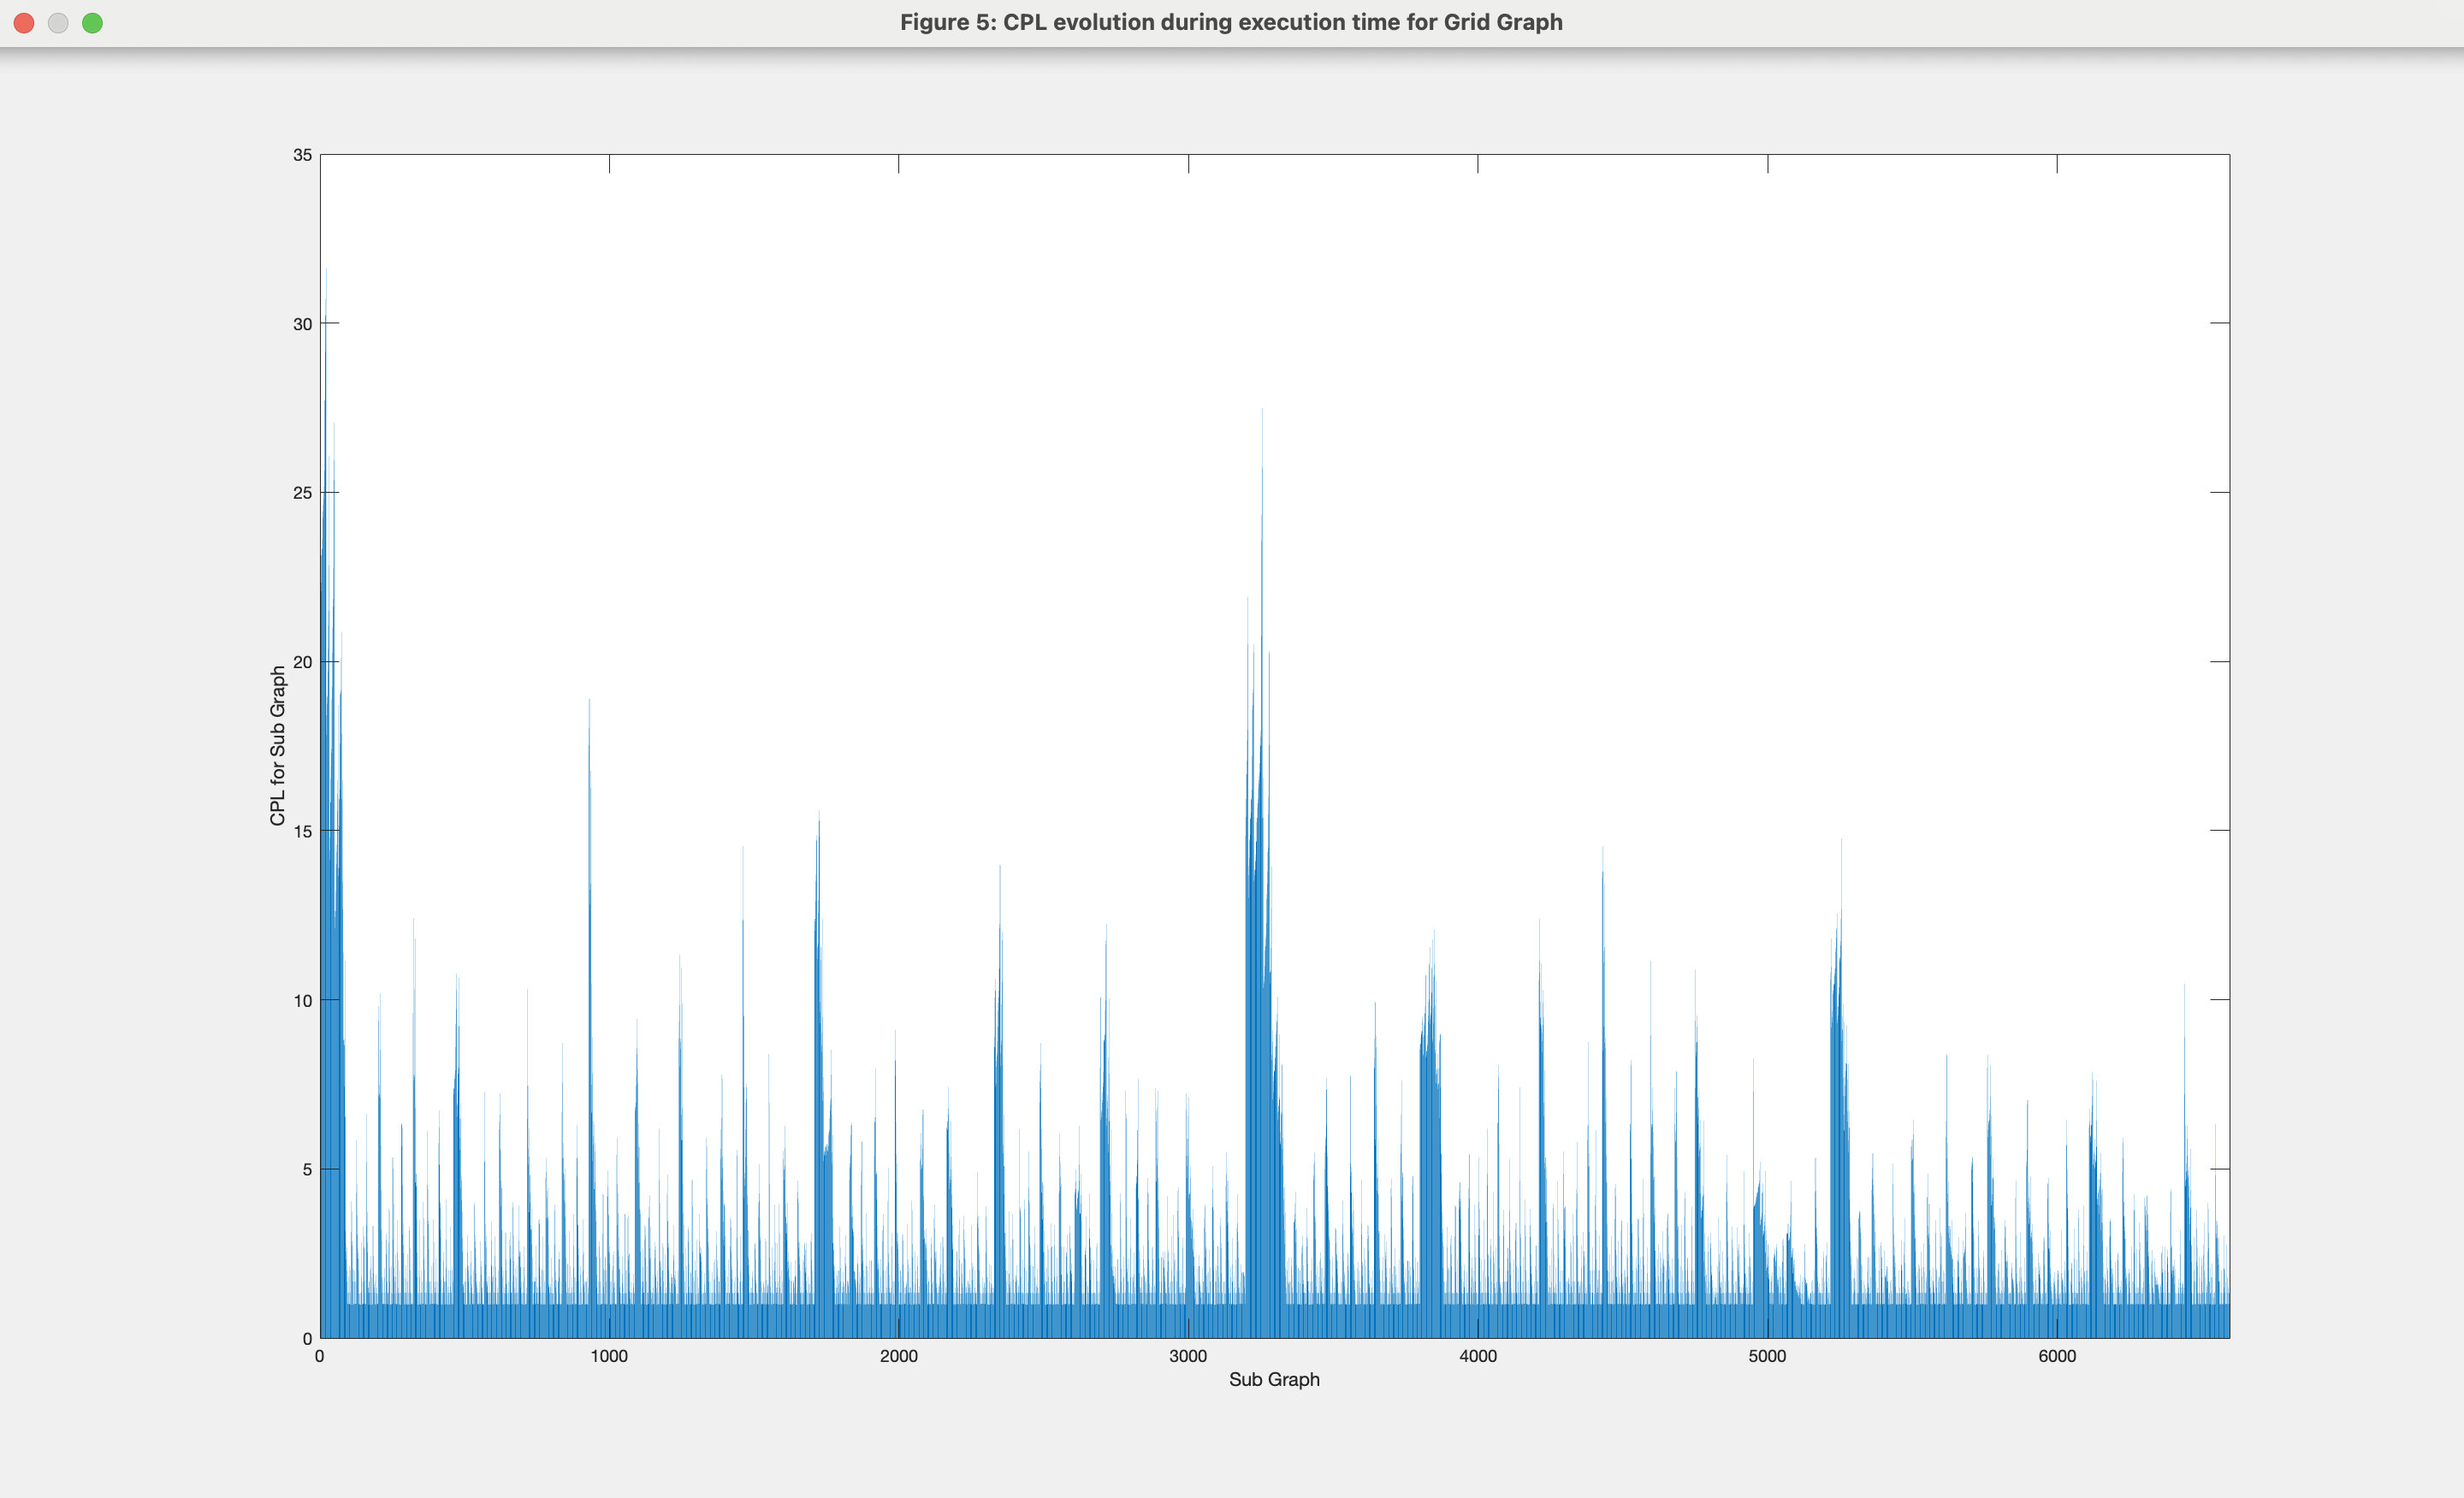
\includegraphics[width=\textwidth]{Figure5.png}\bigbreak
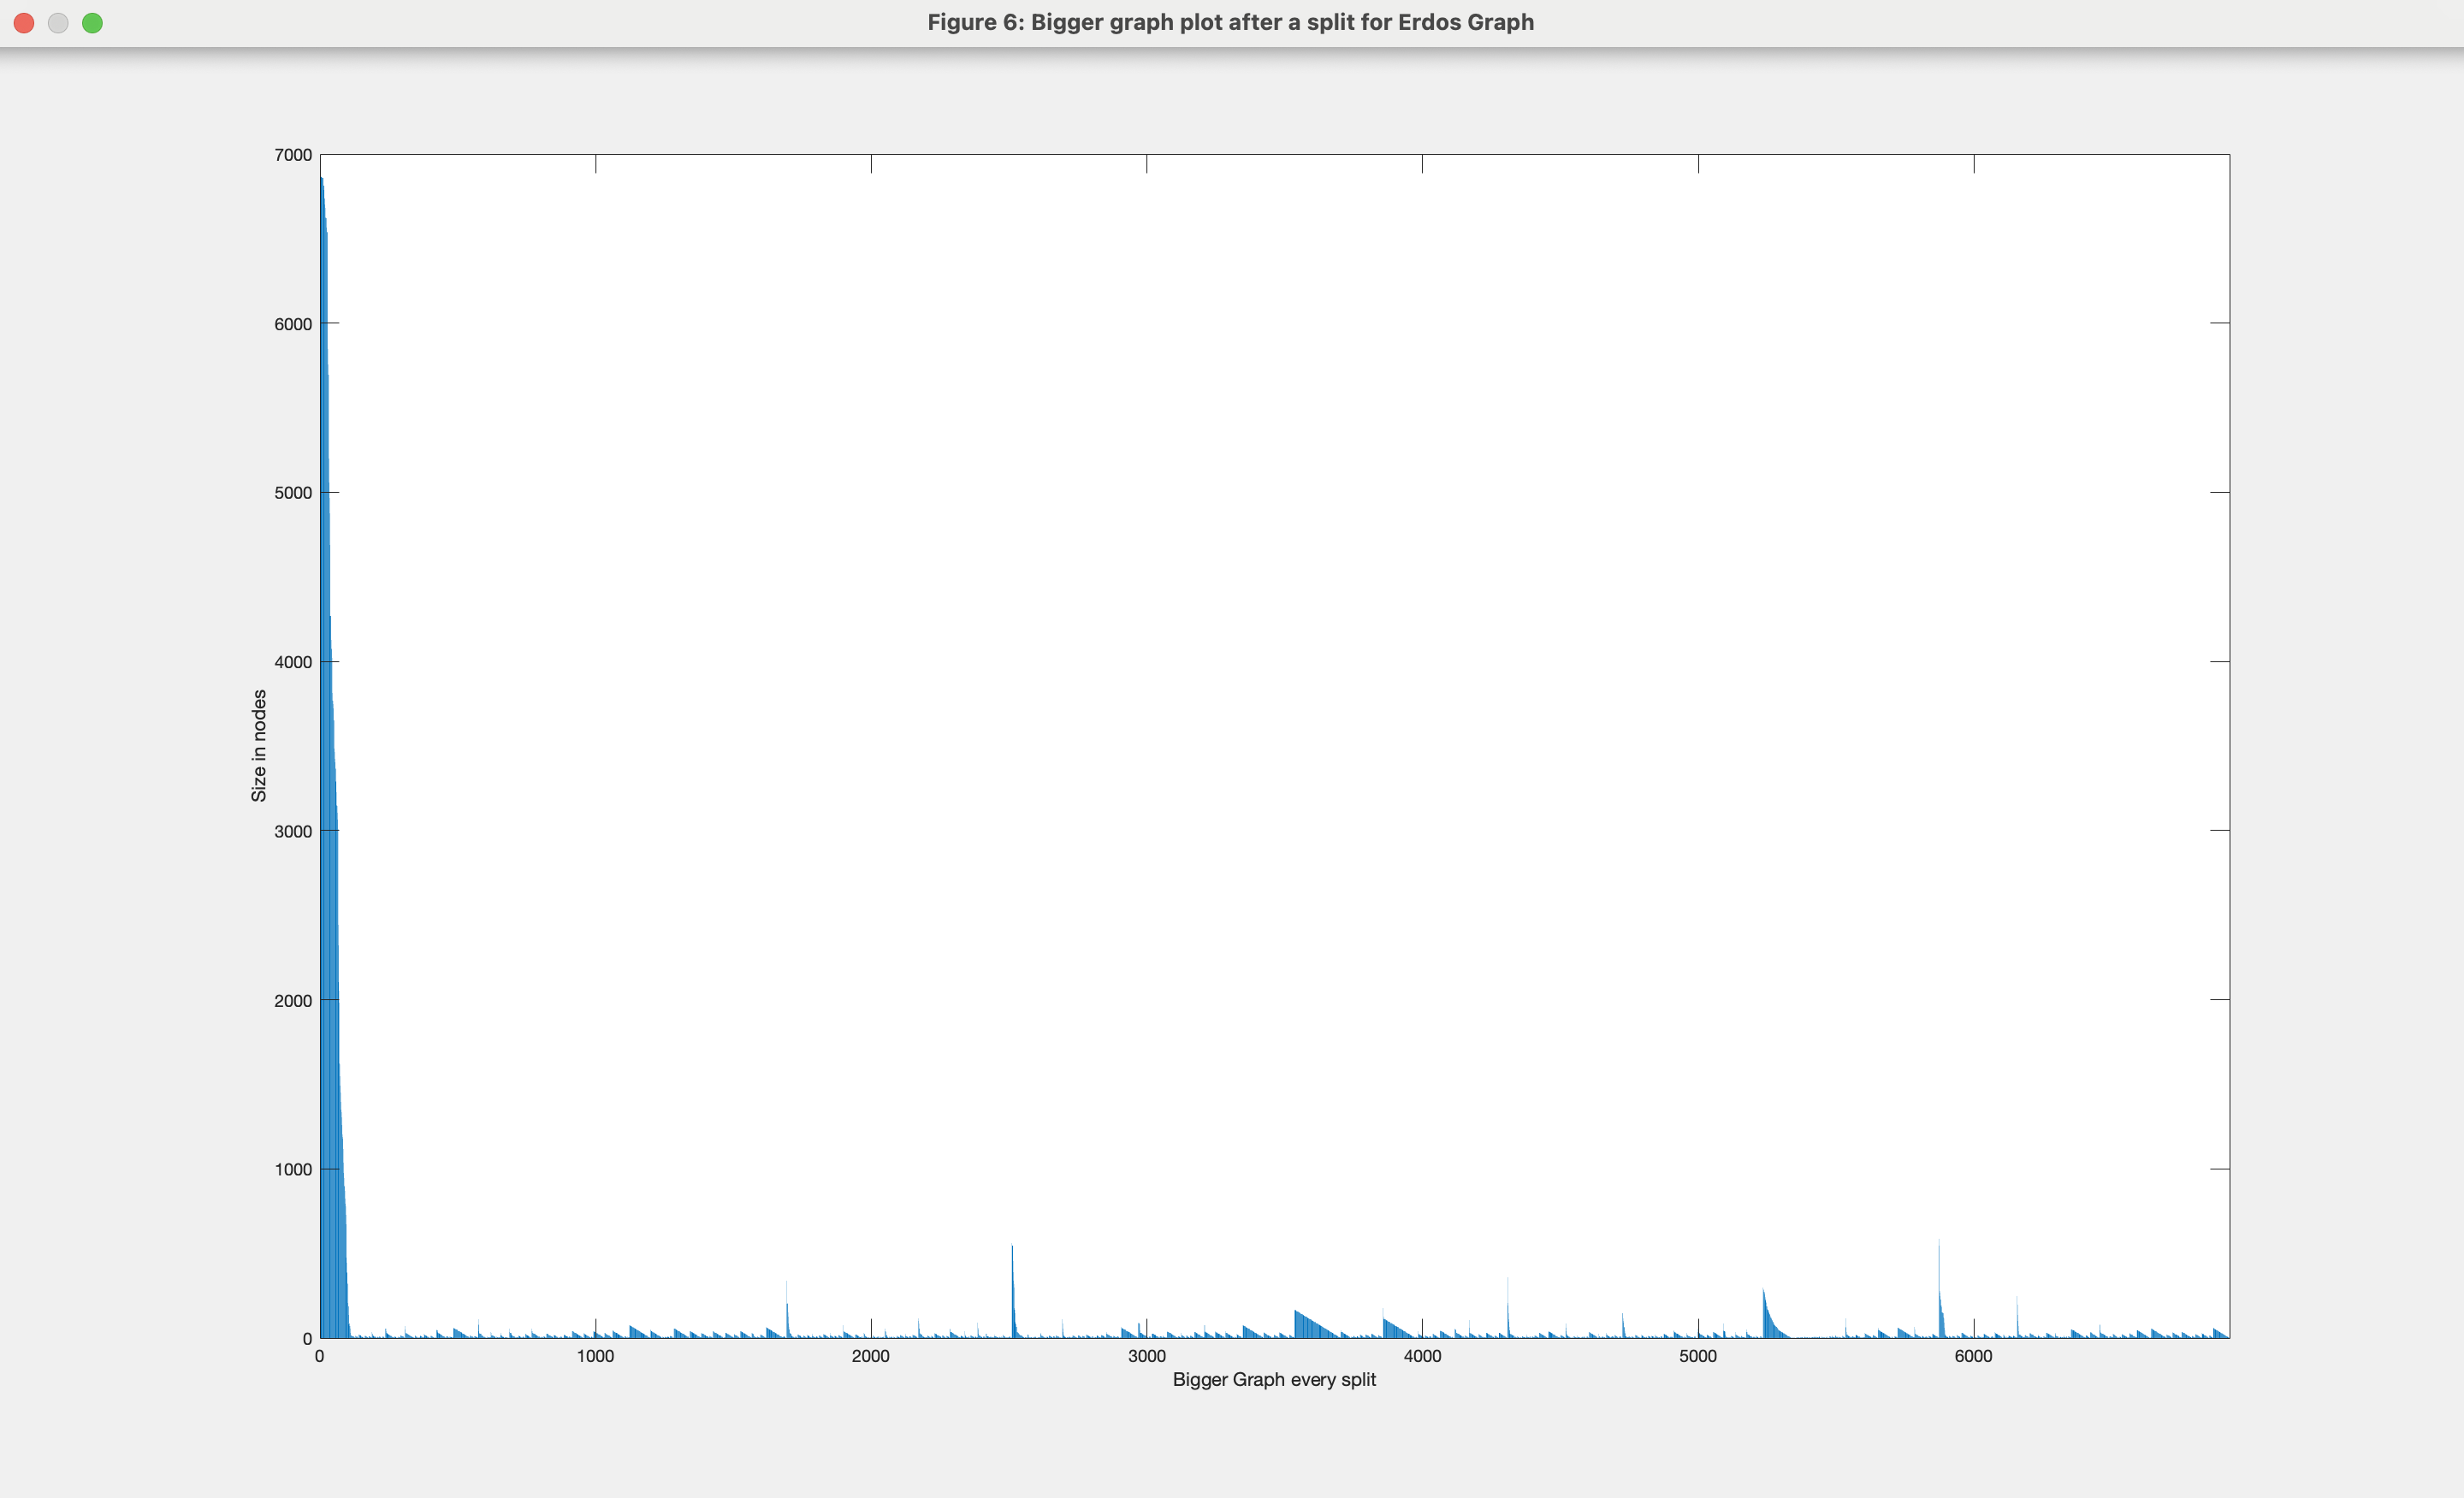
\includegraphics[width=\textwidth]{Figure6.png}\bigbreak
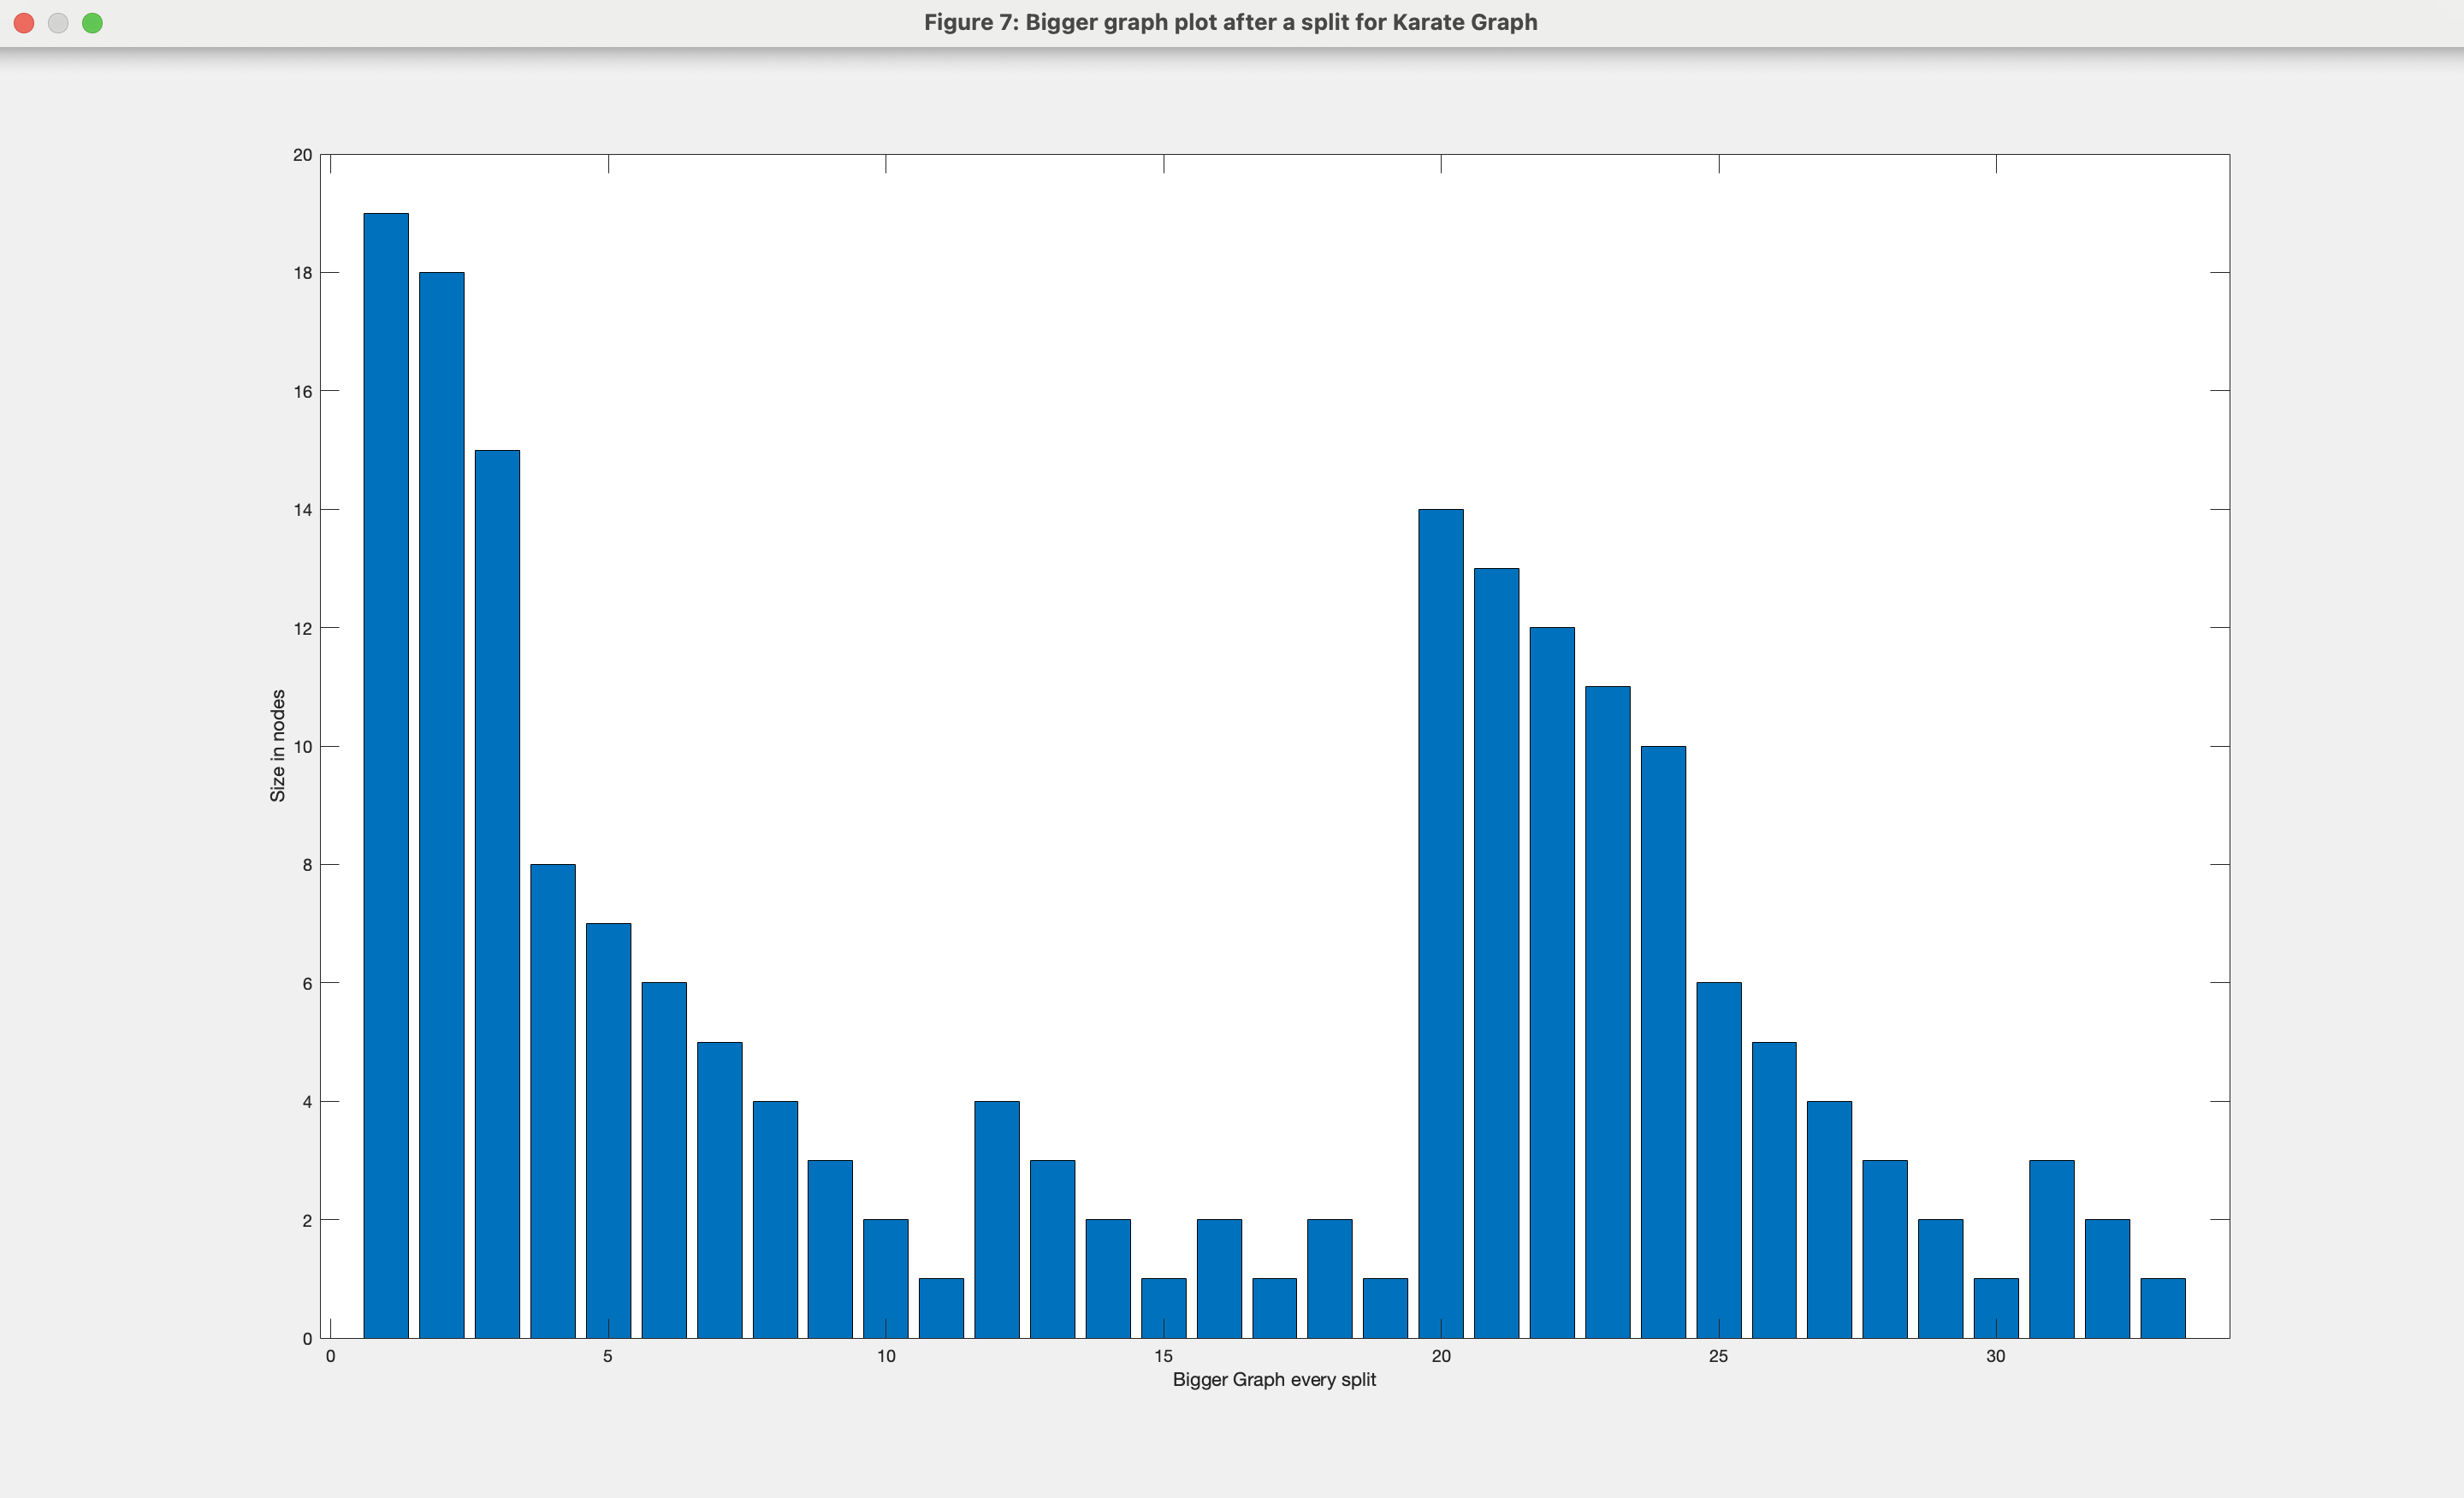
\includegraphics[width=\textwidth]{Figure7.png}\bigbreak
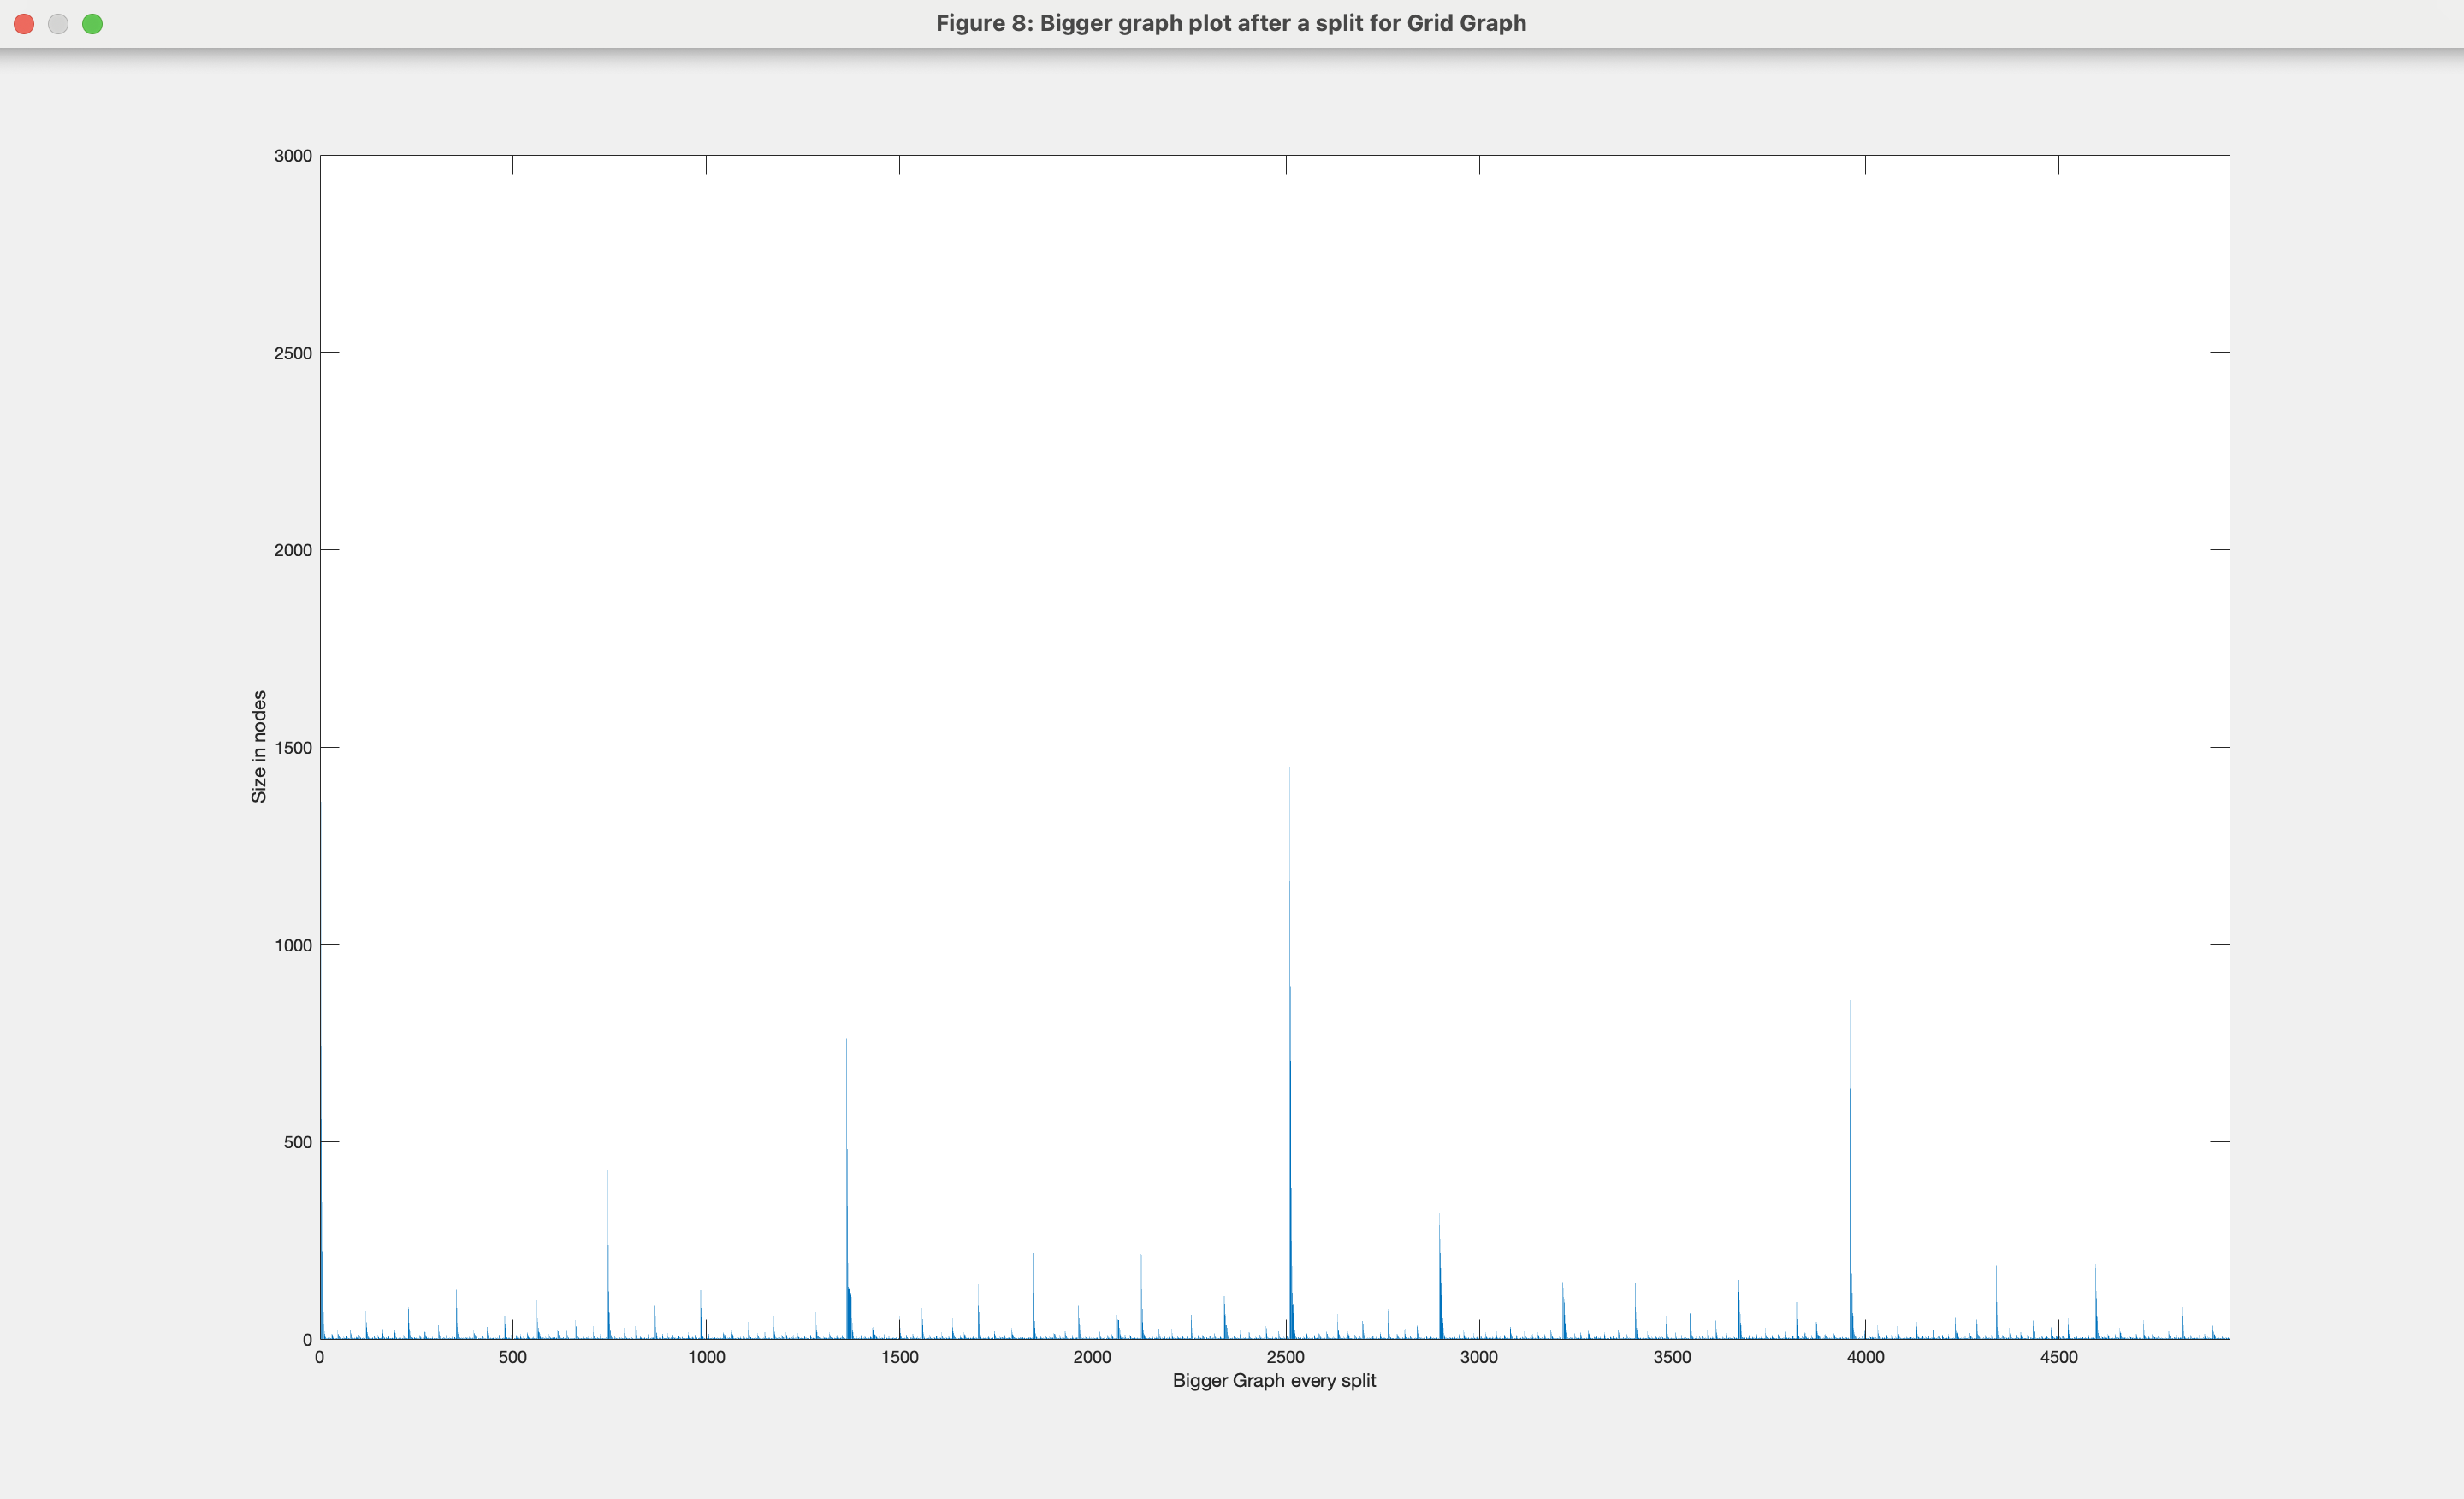
\includegraphics[width=\textwidth]{Figure8.png}\bigbreak
\end{document}